\documentclass[12pt]{amsart}
%%%%%%%%%%%%%%%%%%%%%%%%%%%%%%%%%%%%%%%%%%%%%%%%%%%%%%%%%%%%%%%%%%%%%%%%%%%%%%%%%%%%%%%%%%%%%%%%%%%%%%%%%%%%%%%%%%%%%%%%%%%%%%%%%%%%%%%%%%%%%%%%%%%%%%%%%%%%%%%%%%%%%%%%%%%%%%%%%%%%%%%%%%%%%%%%%%%%%%%%%%%%%%%%%%%%%%%%%%%%%%%%%%%%%%%%%%%%%%%%%%%%%%%%%%%%   
\usepackage{amssymb}
\usepackage{amsmath}  
\usepackage{amsfonts}
\usepackage{mathrsfs}  
\usepackage{graphicx}
\usepackage{color}   
\usepackage[onehalfspacing]{setspace}
\usepackage{ragged2e}  
\justifying     
\usepackage{caption} 
\usepackage{etex} 
\usepackage{longtable} 
\usepackage{graphicx} 
\usepackage{amsmath}
\usepackage{multirow}
\usepackage{setspace}
\usepackage{footmisc}
\usepackage{amssymb}
\usepackage{amsfonts}
\usepackage[font=bf, justification=centering]{caption}
\usepackage{geometry}
\usepackage{float}
\usepackage{verbatim}
\usepackage{array}
\usepackage{booktabs}
\usepackage{pdflscape}
%\usepackage{xy} 
\usepackage{rotating}
\usepackage[round,authoryear]{natbib}
\usepackage{appendix}
\usepackage{lscape}
\usepackage{subcaption}
\usepackage{graphicx}
\usepackage{amsfonts}
\usepackage{placeins}
\usepackage[utf8]{inputenc}
\usepackage{charter}
\usepackage[colorlinks=true,citecolor=blue,urlcolor=blue,pdfpagemode=UseNone,pdfstartview=FitH]{hyperref}
\usepackage{apptools}
%\usepackage{chngcntr}
\usepackage{multibib}
\usepackage{multirow}
\DeclareUnicodeCharacter{00A0}{'}
%\usepackage[capposition=top]{floatrow}
\newcites{main,supp}{References,References}
%\AtAppendix{\counterwithin{lemma}{section}}
\makeatletter
\def\section{\@startsection{section}{1}
	\z@{1.0\linespacing\@plus\linespacing}{.5\linespacing}{\Large}}

\def\subsection{\@startsection{subsection}{2}
	\z@{.8\linespacing\@plus.7\linespacing}{.7\linespacing}{\large}}

\def\subsubsection{\@startsection{subsubsection}{3}
	\z@{.5\linespacing\@plus.7\linespacing}{-.5em}{\normalfont\bfseries}}
\makeatother                   

\setcounter{MaxMatrixCols}{10}
%TCIDATA{OutputFilter=LATEX.DLL}
%TCIDATA{Version=5.50.0.2953}
%TCIDATA{Codepage=936}
%TCIDATA{<META NAME="SaveForMode" CONTENT="1">}
%TCIDATA{BibliographyScheme=Manual}
%TCIDATA{LastRevised=Friday, May 08, 2015 15:13:41}
%TCIDATA{<META NAME="GraphicsSave" CONTENT="32">}
%TCIDATA{Language=American English}

\numberwithin{equation}{section}

\newtheorem{theorem}{Theorem}[section]
\newtheorem{lemma}{Lemma}[section]
\newtheorem{corollary}{Corollary}[section]
\theoremstyle{definition}
\newtheorem{definition}{Definition}[section]

\theoremstyle{definition}
\newtheorem{assumption}{Assumption}[section]

\theoremstyle{definition}
\newtheorem{example}{Example}[section]

\setlength{\textwidth}{6.5in}
\setlength{\textheight}{9in}
\setlength{\topmargin}{-0.1in}
\setlength{\oddsidemargin}{0in}
\setlength{\evensidemargin}{0in}
\vfuzz4pt
\hfuzz4pt
  

\title{}
\begin{document}
	\vspace*{3ex minus 1ex}
	\begin{center}
		\Large \textsc{Love the Candidate but Hate his Party: \\ the Effect of Reelection on Party Dealignment in Mexico} %\\ The Asymmetric Effect of the Removal of Term Limits on Partisan and Personal Incumbency Returns}
		%\bigskip  
	\end{center}
	
	
\date{May 24, 2021} 
\vspace*{3ex minus 1ex}
	\begin{center}
		Rafael Ch\\
		
		\textit{New York University}\\
		
	\end{center}
	 
	\thanks{%I thank Pablo Querubin, Cyrus Samii, Hye Young You, Neal Beck, Jacob Shapiro, Juan F. Vargas, Nicholas Haas, Reed Lei, Lucia Motolinia and participants at the Summer Cohort Seminar, Graduate Political Economy Seminar, and Comparative Politics Seminar at NYU, APSA 2020, SPSA 2021, and MPSA 2021 panelists, as well as the members of the Methods and Data Seminar at the University of Wisconsin-Madison for their amazing comments and suggestions. All mistakes are my own.
	\\
	 \\ \textbf{Ch:} Wilf Family Department of Politics, New York University. \\ Email: \url{rafael.ch@nyu.edu}
	 \\ Website: \url{https://wp.nyu.edu/rafaelch/}}
		  
	\begin{abstract}    
	
A large literature has studied the electoral returns to incumbency. However, the estimated incumbency returns in the majority of studies mask an understudied dynamic between parties and their members: both can be hated, loved or differentially liked by their constituency. These scenarios hold different implications on citizens valuation of the electoral system and the existent accountability dynamics. This paper opens up the black box of incumbency by disentangling the personal and partisan incumbency advantage. To do so, I use a difference-in-discontinuity design of close elections in Mexico that exploits the staggered implementation of a term limit reform that introduced reelection for mayors from 2014 to 2022. Term limit elections allow us to identify a partisan advantage while those with candidates up for reelection identify both the partisan and personal incumbency returns. The difference between them identifies the personal from the partisan effect. The main result shows that races up for reelection experienced an incumbency advantage; however, this hides an asymmetry: a personal incumbency \emph{advantage} is found, while parties suffer from an incumbency \emph{disadvantage}. The research design allows to solve several methodological issues of past studies that have tried to disentangle the partisan from the personal effect, primarily rule out potential pretrends of term limit and non-term limit races, as well as concerns on selection coming from the ability and experience of candidates. Overall, the results suggest the personal advantage to be a driving force of incumbency returns, and how  reelection may lead to party dealignment in party-centered systems like Mexico. 
    
	\medskip
	{\noindent \textsc{Key words: Incumbency Advantage, Reelection, Resources, Candidates Effort, Candidates Quality, Performance in Office.}}

		%{\noindent \textsc{JEL Classification: %D72, D78, H57, O17.}}
	\end{abstract}
	
	\maketitle
	\pagebreak
%%%%%%
%COMMENTS:
%difference between reelection increased accountability and then led to a personal incumbency advantage or reelection allows us to tease the personal from the incumbency advantage. So technically I can´t test the first: we don´t have a control group for that. So what I can say is that reelection led to an incumbency disadvantage. But this is explained by an asymmetric effect that points to dealingment. This is how I should write the paper. 
\begin{comment}
Figures:
\begin{enumerate}
\item Main effect on incumbency disadvantage
\item Asymmetric effect
\item Identification
\item Robustness 
\item Why?

\end{enumerate}	

So motivation:
1. Positive and negative incumbency advantage have been identified. But this unmasks the asymmetry. 
2. It has been challenging

Introduction
1. Positive and negative inc. advantages. 
2. Multiple are the reasons. 
3. This are confounded by not differentiating the personal from the partisan incumbency advantage. 
4. This is methodologically challenging
5. Use term limit reform to explore this. 
6. Find a negative incumbency advantage of reelection which could be wrongly interpreted as if reelection damages the electoral connection. 
7. But explained by an assymmetry. 
8. Speaks to the literature of dealingment
9. speaks to other contributions

Theory:
1. incumbency advantage
2. but some are party and some are candidate driven. How to know?
3. Personal vs partisan inc. advantage
4. Mexico' incumbency advantage

%Methods to study this: redistricting by ansolabehere_snyder_2000

\end{comment}
   
\clearpage
\section{Introduction}

Over the past decades, an important theoretical and empirical literature has shown that incumbents may enjoy an electoral advantage \citep{ashworth_2012, cox_morgensten_1993, cox_katz_1996, ansolabehere_snyder_2000, ashworth_bdm_2008, ashworth_etal_2019} or suffer from an electoral disadvantage in the next election \citep{klasnja_2015, klasnja_titiunik_2017}. However, whether positive or negative, the electoral returns from incumbency mask an understudied dynamic between the returns associated to parties and those exclusively of candidates. Disentangling both measures is important to understand citizens valuation of the electoral system and the existent accountability dynamics \citep{mayhew_1974, fowler_hall_2014}. For instance, a partisan incumbency advantage might imply that voters believe parties control candidates behaviors, and thus would allow parties to hold a credible threat against renegade candidates. The implications for a personal advantage are different, however: a personal advantage makes candidates vital for parties electoral success, leading the latter to allow more leeway to the former since retiring or switching parties may hurt parties electoral success. However, the implications of a personal advantage are different from the partisan one. A positive personal advantage makes retiring politicians support of new candidates vital for their electoral success, and stepping down or switching parties may hurt their parties in the next election.\footnote{Likewise, a partisan incumbency disadvantage may imply citizens like partisan balance across time and may create incentives for candidates to differentiate themselves from their parties \citep{klasnja_titiunik_2017}. Contrastingly, a negative personal advantage may lead parties to differentiate themselves from candidates and stop their electoral support to them or retire the nomination in the next election.} Moreover, if a personal (partisan) effect exists and the partisan (personal) one is negligible it implies voters attribute actions in office to candidates (parties) and not their parties (candidates) or that a party (personal) dealignment might be taking place \citep{cox_katz_1996}.   
   
However, uncovering the partisan and personal incumbency advantage has proved methodologically challenging: every time a candidate is an incumbent so is its party so we cannot uncover the personal from the partisan incumbency return. As a consequence, the personal incumbency advantage is biased (upwardly or downwardly) to changes in the partisan incumbency effects. This is true with the most widely used method to estimate the returns to incumbency, the regression discontinuity design (RDD) of close elections, that conflates the personal and partisan incumbency advantage, even when the variables are defined in partisan terms (such as likelihood of the party winning or the party vote share) \citep{fowler_hall_2014}. To overcome these obstacles studies have tried to exploit cross-sectional comparisons between term limit and non-term limit races \citep{gelman_king_1990}, expiring and non-expiring careers \citep{fowler_hall_2014}, and changes in redistricting \citep{ansolabehere_etal_2000, desposato_petrocik_2003, sekhon_titiunik_2012}. However, for identification they have relied on strong assumptions such as no differential pretrends in incumbency returns \citep{fowler_hall_2014, ansolabehere_snyder_2004}. %when comparing term-limit and non-term limit elections or expiring vs. non-expiring races  
Moreover,  while studies have used RDDs to rule out potential omitted variable bias coming from the correlation between current and future electoral success including parties reputation and candidates type \citep{klasnja_titiunik_2017}, recent evidence points that differences on the quality of incumbents and challengers -the so called scare-off effect- are still present \citep{eggers_2017}. 

This paper identifies the partisan and personal electoral returns to incumbency and solves the existent methodological difficulties faced by the literature. To do so, I use a difference-in-discontinuity of close elections design that exploits the 2014 Electoral Reform in Mexico that introduced reelection for mayors for the first time. The reform was staggered at the state level which allows us to compare the municipal elections in the not-yet-treated states where term limits exist to those in municipalities where incumbents have the possibility to reelect. Term limit incumbency returns identify the partisan effect as candidates cannot run again for office, while the non-term limit incumbency advantage identifies both the personal and partisan advantages. By differentiating both measures we are able to disentangle the personal from the partisan effect. The difference-in-discontinuity design allows us to test for parallel trends prior to treatment. Furthermore, by focusing on close elections we rule out potential omitted variables coming from differences in parties and electoral races. Additionally, this paper compares incumbents in their first term only which allows to rule out important endogenous concerns, particularly those arising from selection such as the difference in the ability or experience of incumbents \citep{ferraz_finan_2008, ferraz_finan_2011}. Lastly, I test for quality differences among incumbents in term limit and non-term limit races, as well as differences between incumbents and challengers to test if quality differences are present. 
 

Results show that the introduction of reelection generated an incumbency disadvantage, i.e., incumbents with the possibility to seek reelection hold a decreasing likelihood to win office in the next election relative to municipalities where candidates are term limited. The same result is found by a decreasing vote share in the next election as a measure for incumbency returns instead of the probability of winning office. However, this incumbency disadvantage masks an asymmetric effect. The incumbency disadvantage is a weighted average of a personal incumbency \emph{advantage} and a partisan incumbency \emph{disadvantage}. This implies incumbency became a personal affair when reelection was introduced in a country with a historically strong party-centered system, Mexico. Results also imply that if candidates retire or switch parties they will hurt the reelection chances of their parties. Not surprisingly, Mexico's 2014 Term Limit Reform introduced a ``party lock'' where mayors who wish to reelected cannot switch parties.  

To address  methodological concerns, the results are not explained by pre-trends in incumbency advantage or heterogeneous treatment effects between different treated cohorts. Results are robust to various specifications, including varying the bandwidth for close elections and the functional form. Moreover no sorting into treatment or manipulation is found when running the typical McCrary test and testing for no discontinuous jump of other covariates at the winning margin threshold. 

The paper then explores the reasons behind the observed incumbency returns. I do not find evidence on quality-based incumbency advantage as there are no differences in the quality of term limited and non-term limited incumbents as measured by their education level. I do find evidence, however, of a resource based incumbency advantage where incumbents up for reelection increase the level of municipal revenues, and received an increase in federal and state fiscal transfers relative to term limit incumbents. A personal incumbency advantage may be explained by citizens expecting a higher budget or transfer in the future which they accrue directly to the effort of the incumbent rather than his party. Interestingly, we also observe a decrease in municipal expenses in social development, infrastructure and public security, and a decrease in the percentage of municipal budget spending (\emph{subejercicios} in Spanish). This could be evidence of how a personal incumbency advantage leads ``incumbents use their office to insulate themselves from electoral pressure'' (\citet{eggers_2017}. 1) and decrease overall spending to focus on particularistic transfers.

The main results of this paper coincide with those of \citep{fowler_hall_2014}, albeit for a different setting. They find that for the U.S. state legislatures the personal advantage is larger than found in previous literature, and that the partisan advantage is zero and possibly negative, as this paper does. This paper is the first one to compare party and personal advantage outside of the US. Moreover, while \citet{fowler_hall_2014} need to assume no pretrends prior to treatment for identification, the difference-in-difference design allows us to test it and rule it out. 

This paper contributes to the literature on incumbency advantage in party-centered systems. A negative partisan incumbency return and positive personal one affects the way we think about parties-members relationships. Even in the case with strong party systems and a party-lock where candidates cannot run for reelection for other parties, parties cannot credibly threaten to withdraw their support from renegade members. In other words, the introduction of reelection debilitates parties power even in party-centered systems like Mexico generating candidate-centered electoral contests. This goes in line with the partisan dealignment as a result of reelection, as the one seen in the electorate of the U.S in the post-war era  \citep{cox_katz_1996}. It also introduced the possibility of new strategic politicians that may work to generate their own incumbency advantage  \citep{mayhew_1974, mckelvey_riezman_1992}.  
 

Lastly, this work is closely related to the incumbency disadvantage literature, particularly the work of \citet{klasnja_titiunik_2017}. This paper borrows their measure of party-level incumbency advantage. However, contrary to their setting that studies a weak party system (Brazil) I explore a strong one (Mexico).\footnote{\citet{klasnja_titiunik_2017} classify Mexico as having a weak political party system. Given Mexico's institutional characteristics and historical legacies I believe this to be a misinterpretation.}

The next section delves into the importance of disentangling the personal from the partisan incumbency returns. I then describe the research design, followed by a brief overview of Mexico's 2014 Electoral Reform and data collection. Empirical results are then presented as well as a section with the mechanisms behind the observed incumbency returns. I close with a discussion on parties-members relationships when asymmetric personal and partisan incumbency returns are present. 


\section{Personal and Partisan Incumbency Advantage}

``Incumbency advantage is the additional electoral support a candidate gains due to his or her incumbent status'' (\citet{cox_morgensten_1993, p. 329}). It can be measured as either the difference in the vote share received by the incumbent in $t+1$ from the vote share perceived at $t$ or the difference in the likelihood of winning office. The literature has found several reasons behind an incumbency advantage from resources, visibility and power gained in office \citep{mayhew_1974, fiorina_1989, king_1991, cox_morgensten_1993}, to differences in the quality of incumbents and challengers \citep{cox_katz_1996, levitt_wolfram_1997, ansolabehere_snyder_2000, eggers_2017}, and the role of information on incumbent's ability and competence to voters \citep{ashworth_bdm_2008, ashworth_etal_2019}. On the other hand, incumbency disadvantage occurs if voters seek to balance power, they dislike parties, or prefer change  \citep{fowler_hall_2014, eggers_2017}, if candidates who replace incumbents or if challengers are of lower quality \citep{eggers_2017}, and/or if parties are weak to control candidates behavior and thus are punished by voters in the following election \citep{klasnja_titiunik_2017}.

Incumbency advantage can be decomposed into two concepts that allow for a better understanding on the relationship between voters, parties and their members: the partisan and the personal incumbency advantage. The partisan incumbency advantages is “the electoral benefit accruing to non-incumbent candidates by virtue of being from the incumbent party” (\citet{fowler_hall_2014}, p. 501). In other words, it speaks to the support parties win in the next election due to their incumbent status. The personal incumbency advantage, however, is a different concept: it is defined as the returns to incumbency that make a candidate better off as an incumbent relative to a candidate for an open seat \citep{fowler_hall_2014}. As such, the personal incumbency advantage has been the typical measure of returns to incumbency in the literature. However, when incumbency returns are estimated the personal advantage is always conflated with the partisan advantage as parties and candidates are incumbents at the same time. 

Consider, for instance, the experiment described by \citet{lee_2008}. He states that in the case of US elections, ''[t]he ideal thought experiment for measuring the incumbency advantage would exogenously change the incumbent party in a district from, for example, Republican to Democrat, while keeping all other factors constant. The corresponding increase in Democrat electoral success in the next election would represent the overall electoral benefit due to being the incumbent party in the district" (p. 683). To proxy for this thought experiment, \citet{lee_2008} runs an RDD of close elections comparing the returns to incumbency in $t+1$ for incumbents who barely win to those that barely lost at $t$. However, the resulting incumbency returns provide an entangled average effect of both the personal and partisan incumbency return. Moreover, experiments such as this tend to interpret the results as accruing solely to incumbents rather than their parties, and do not consider voters may value differentially parties and their representatives. 

Substantively, these two concepts provide different interpretations of the electoral system. Overall there are six possibilities. First, we can observe a  partisan and personal incumbency \emph{advantage}. In such case high reelection rates increase the concern that incumbents may insulate themselves from electoral threats, and debilitate their accountability to constituents \citep{ashworth_etal_2019, cox_katz_2002}. Parties might not have incentives to monitor or exercise control over their members given their electoral isolation as well as the potential negative consequences of standing against incumbents with high personal electoral returns from office. Overall, a personal and partisan incumbency advantage may signal that voters accrue actions of candidates to both parties and representatives, and may lead parties and candidates to isolate from the electoral connection created by reelection \citep{mayhew_1974}. 

 In a second scenario, we can observe both a partisan and personal incumbency \emph{disadvantage}. A negative partisan incumbency may show constituents prefer partisan balance \citep{folke_snyder_2012}, believe the ``grass-is-greener'' with other parties \citep{bhatia_turan_2013}, or dislike institutions relative to their members \citep{parker_davidson_1979}, for example. A negative personal incumbency might signal voters see incumbent politicians as too corrupt and prefer new candidates to hold office in the next turn. In this setting, parties choice might be to nominate new candidates to contend for office despite incumbents holding the possibility to reelect. Incumbents up for reelection may choose to switch parties or run for other political positions at the state or federal level and not run for reelection. 
  
 Third, we can observe an asymmetry where a personal incumbency \emph{advantage} might coincide with a partisan incumbency \emph{disadvantage}. Parties no longer hold a credible threat to punish renegade incumbents. Moreover, candidates hold incentives to differentiate themselves from their parties through various personalistic strategies as voters may attribute the actions of candidates only to them and not their parties. A positive personal incumbency might also imply voters transfer their support to an incumbents co-partisan o whomever the current incumbent wishes to endorse if they are retiring. 
  
 
 Fourth, an asymmetry with a personal incumbency \emph{disadvantage} might coexist with a partisan incumbency \emph{advantage}. In this case, citizens may attribute actions of candidates to their parties considering them as lame ducks in office. In this setting we may also have that retiring incumbents are not invited to support new candidates from their party as this may damage their electoral success in the coming election. More importantly, this scenario makes elections party-centered rather than candidate-centered, with parties holding a credible threat to withdraw their support or nomination for dissident members since new candidates will benefit from the positive partisan electoral return for the next election.  

Additional scenarios are for either partisan or personal incumbency returns to be negligible. When the personal incumbency is not different from zero, it may imply that actions of incumbents do not affect the parties return from incumbency if they choose to step aside by switching parties or retiring. On the contrary, a negligible partisan incumbency return makes the branding and attributes of parties not as important for voters even if they rely on partisan labels to define their vote. Moreover, voters in this setting might see the actions of incumbents as separate from their parties \citep{fowler_hall_2014}. 

A negligible partisan incumbency return and a positive personal incumbency is strongly tied to the large literature on partisan dealignment in the United States. As \citet{beck_1985} notes, an electorate that appears to be highly partisan may be just a facade if ``partisanship is merely an expression of momentary vote choice'' (p. 233). This dealignment trend has been identified in the US since the 1953 due to generational changes \citep{beck_1977, norpoth_rusk_1982}, characterized by the weakening of group bases of party support and increase electoral competition, in Britain since 1970 due to retrospective voting \citep{alt_1977}, the Netherlands since the late 1960s due to vote switching and the decline in political cohesion of groups \citep{irwin_dittrich} and Denmark, Norway and Sweden were class voting declined since the 1970s \citep{borre_1995}. In Mexico -the study case at hand in this paper-, winning margins have substantively declined since the move to democracy in 2000, while party bases have constantly migrated from one party to another, and from one political leader to another, for example. Besides the case of the US, however, partisanship has been linked too closely to candidate vote choice to assess whether dealignment ocurrs.  However, the existence of a strong personal incumbency advantage relative to a negligible or small partisan one may clearly portray a dealignment of citizens from mass politics. 
   
As described thus far, evaluating an electoral system requires the identification of the personal and partisan incumbency returns. Limiting to the former provides and incomplete picture of the dynamics between voters, parties and their members. 

Take for example the case of Mexico. Prior to the introduction of the 2014 Term Limit Reform, Mexico had a party-level incumbency disadvantage. With term limits in place, the likelihood of incumbent parties to win office in the next election where negative and close to 28\% according to \citet{klasnja_titiunik_2017} who take into account all mayoral elections from 1997 to 2009. Appendix \ref{appendix:rdd} runs a similar experiment with an RDD with close elections and optimal bandwidths following \citet{calonicoetal_2014} but considering all mayoral races from 1989 to 2018. Furthermore, I run to separate RDDs for whether they had term limits or not due to the introduction of reelection by the 2014 Electoral Reform. I find an incumbency disadvantage of 11\% significant to the 1\% level, using both a linear and quadratic polynomial. An incumbency disadvantage is also found using vote share, of -4\% significant to the 1\% level using a linear and quadratic polynomial as well. Contrastingly, for elections that removed term limits and introduced reelection for mayors we observe a positive but not significant effect on incumbency returns, using both the probability of victory or the winning margin in the next election. In other words, it seems reelection erased the negative returns to parties in Mexico. However, these incumbency returns estimates do not allow us to assess whether incumbency became a personal matter when reelection was introduced or remained mainly a partisan one. In other words, we are unable to securely state that Mexico moved from a party to a candidate centered system due to introduction of reelection and the strengthening of voter accountability, and what this implies in terms of of voters, parties, and representatives dynamics.

 Moreover, these estimates may be biased in two ways. First, by comparing term limit and non-term limit elections we need to assume there are parallel trends which might not be the case and an RDD does not allow us to test this assumption. Furthermore, as \citet{eggers_2017} notes even when comparing close elections in a regression discontinuity design, a potential difference in the quality of incumbents and challengers may still exist. The next section addresses these methodological issues by describing the research design used in the paper.  
 

%\section{Term Limits and Reelection}

%Removing incumbents via term limits increases competition because the electoral advantage dissipates rather than affecting the future candidate of the party. 

\section{Research Design to Disentangle the Personal from the Partisan Incumbency Advantage}
The typical methodological tool to study incumbency returns is the regression discontinuity design (RDD) \citep{thistlethwaite_etal_1960, imbens_lemieux_2008, lee_2008}. Since election results are not exogenous, we move to a local environment where we compare very close elections. Presumably, by comparing incumbents that barely won to those that barely lost we have identical candidates and parties on each side of the cutoff \citep{lee_2008, boas_hidalgo_2011, broockman_2009, butler_2009, dalbo_etal_2009, querubin_snyder_2013, titiunik_2012, klasnja_titiunik_2017}. However, recent evidence shows that even with RDDs of close elections barely winners and losers might differ in terms of quality \citep{eggers_2017, caughey_sekhon_2011, grimmer_etal_2012}. Problems include incumbents being better than challengers or a potential scare-off effect of challengers. 

RDDs, moreover, cannot disentangle the personal and party incumbency advantage. As \citet{erikson_titiunik_2015} show, the RDD coefficient is defined as 2*Partisan Advantage + 2*Pr(Winner Runs Again)*Personal Advantage. This makes the partisan and personal advantage unidentified. A possibility to disentangle them is to compare two different regression discontinuity models, one for elections with term limits where no candidate can remain in office more than the appointed term, and one for elections with the possibility to reelect at least one term. \citet{fowler_hall_2014} show that the difference between these two models yields the personal incumbency advantage, since the term limit one captures the partisan effect and the non-term limited model the partisan and personal effect \citep{gelman_2011}. For this difference to yield identified personal and partisan effects, however, we need to rely on three identification assumptions. First, as with any RDD of close elections, that potential outcomes are continuous at the forcing variable threshold, i.e. the electoral vote share. This implies that the current and next election support the same parties in contestation. The second assumption states that the average personal and partisan incumbency advantages in a given election do not vary differently across time for those with and without term limits. This assumption is the typical parallel trend assumption in difference-in-difference (DiD) designs. As with DiDs, the parallel trend assumption does not imply that term limit and non-term limit elections are the same across covariates, but that the vary similarly across time prior to treatment. However, in the case of RDDs it is a very strong and non-testable assumption. \citet{fowler_hall_2014} rely on various tests to assess this assumption including comparing legislative elections in states with term limits and without, the latter being a placebo. However, state legislatures vary in different characteristics across time such as the quality of challengers and potential scare-off effects \citep{rogers_2014}. The third identification assumption is that there is no change in the quality of incumbents when an incumbent retires as is replaced by a new candidate. 


Other papers have tried to disentangle the personal from the partisan incumbency advantage. By definition, a personal incumbency advantage comes from comparing the electoral returns of an incumbent up for reelection to the same seat -in the same election and locality at the same time- but with term limits. This makes the open seat a counterfactual scenario. A similar experiment in mind is that of \citep{gelman_king_1990} that compares two scenarios, one where the incumbent legislator runs, and another when it retires, and both accrue to the same party. Holding the party constant allows to tease the party incumbency advantage. Another experiment has exploited redistricting, where the personal incumbency return comes from comparing  new voters who are first experiencing and incumbent are compared to old voters who already know the incumbent \citep{sekhon_titiunik_2012}. The problem, however, is that even conditional on covariates old and new voters may differ introducing potential bias as noted by a large gerrymandering literature. 

To overcome these empirical challenges and relax the  assumptions to identify the personal and partisan incumbency advantage, I leverage a difference-in-discontinuity design that exploits the staggered rollout of an Electoral Reform in Mexico in 2014 that removed term limits and compares only mayoral close elections. Term limited incumbents are forced to retire but not their parties allowing to identify a partisan incumbency advantage. Meanwhile, candidates facing reelection enjoy the perks of their party also running for reelection. The difference between the average probability of winning in $t+1$ (or vote shares) of those competing in term limited elections relative to non-term limited ones in $t$ would provide an unbiased estimate of the personal (A) and partisan incumbency advantage (B). Meanwhile, the effect of term-limit races would provided an unbiased estimate of the partisan incumbency advantage (B). By differentiating these two quantities (A+B-B=A) we can obtain an unbiased estimate of the personal incumbency advantage. Importantly, this quantity needs to be divided by 2 and take into account the probability of an incumbent running again for office as some may retire. As described by \citet{fowler_hall_2014} making a reference to the findings of \citet{erikson_titiunik_2015} ``the partisan incumbency advantage is doubled because the winning party has both the benefit of being the incumbent party and the benefit of the other party not having this advantage. Similarly, if we knew that the winner of the first election would always run for re-election, then the RD estimate would also include two times the personal incumbency advantage. However, the incumbent does not always seek re-election, so we must multiply this term by the probability that the winner of a close election seeks re-election'' (p. 512). The diff-in-discontinuity of close elections design allows us to test for parallel trends instead of assuming such trends exist prior to treatment as other studies do.

Furthermore, in this paper instead of assuming that the quality of an incumbent that retires is similar to that of the new candidate, I test whether we observe quality differences in incumbents that barely won in term limited and non-term limited electoral races. Also, by comparing first term to second term incumbents in both term limit and non-term limit elections I test whether a potential scare-off effect exists, i.e. the tendency of incumbents to deter strong challengers. Presumably this is a good way to test the scare-off effect since challengers would be more concerned of facing an incumbent in its second term given the increase in experience rather than those in their first term. 

Lastly, the main research design only compares first term mayors in term limit and non-term limit races. The introduction of reelection for the first time allows for this comparison and erase the concern on differences between experience or ability between candidates up for reelection or bounded by term limits \citep{ferraz_finan_2008, ferraz_finan_2011}. For clarity, the next subsection provides a description of the 2014 Term Limit Reform in Mexico.  

\subsection{Mexico's 2014 Term Limi Reform}

Since 1993 in Mexico, the Partido Nacional Revolucionario (PNR and former PRI) imposed an 80-year old ban on reelection making all presidential, gubernatorial, legislative and mayoral elections term limited. The motivations behind this constitutional amendment was to control self-motivated politicians to deviate from the party line in any of the multi-level party structure. The famous phrase in Mexican politics ``if you move you don't appear in the photo'' (\emph{si te mueves no apareces en la foto}) shows the spirit of the PNR and later the PRI to weaken  local party bosses and allow the party to control political careers at the federal, state and local level by limiting reelection \citep{weldon_2003}. 

   
However, in February 2014, the Mexican Federal Congress approved the Electoral Reform that municipal mayors to reelect for at least two electoral periods.\footnote{The reform also introduced reelection for local and federal legislators who are allowed to reelected up to 4 consecutive terms.} %%% Some story here

Besides the removal of term limits for mayoral races, the reform included the creation of the National Elections Institute to rule all elections in the country as well as the introduction of a ``party lock'' which constrained incumbents from running for reelection with other parties. 


State legislatures, mostly under control of governors, were granted discretion to define the number of terms for both legislators and mayors. While variation in the number of terms exists at the state-legislator level \citep{motolinia_2020}, all state legislators approved up to 2 consecutive reelection terms for mayors except for the case of Hidalgo, Nayarit, Tlaxcala and Veracruz that allowed candidates' reelection, but not consecutively, bypassing the reform.  

\begin{figure}[h]   
\centering 
\caption{Mexican States Electoral Reform Treatment Status}
\label{fig:treatment_status}
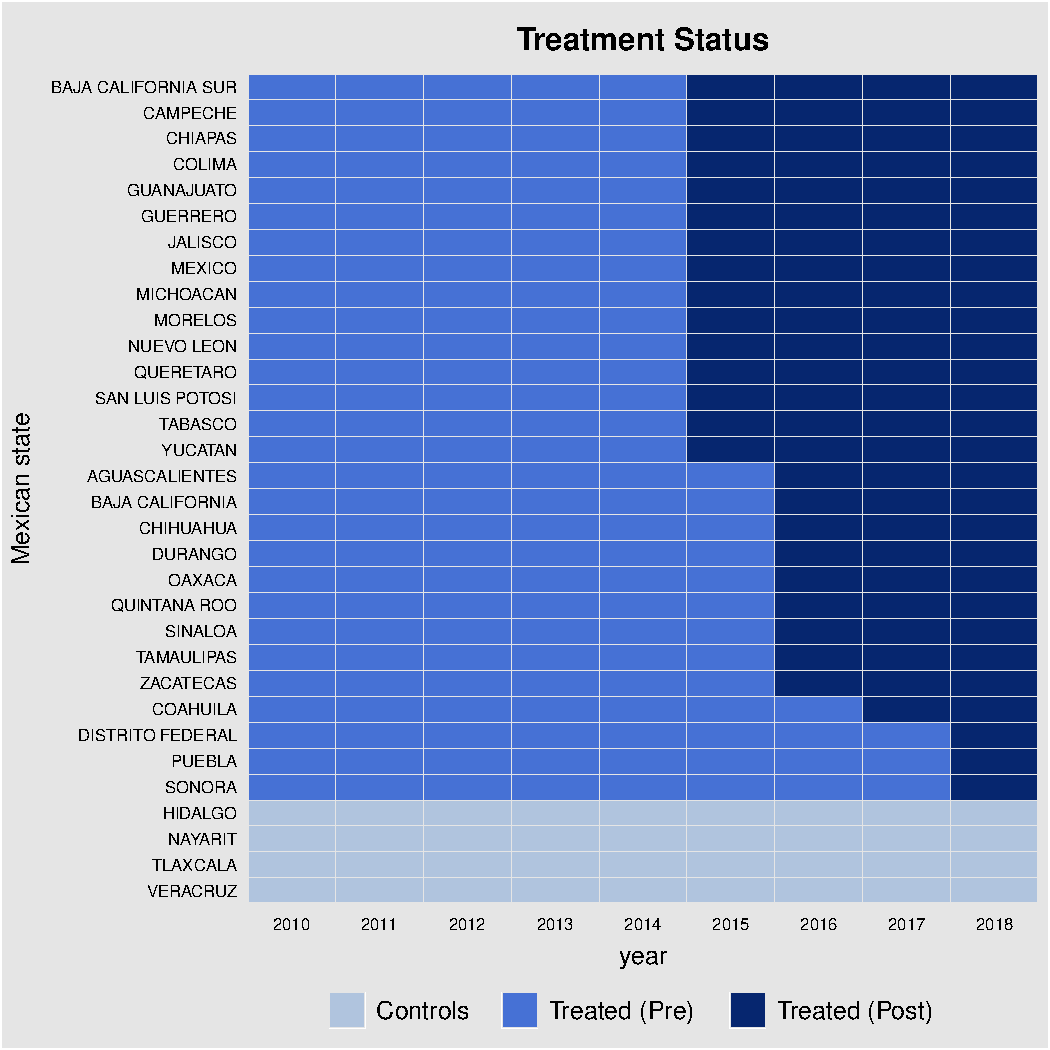
\includegraphics[width=0.75\textwidth]{../Figures_incumbency/reform_treatmentstatus.pdf}     
\captionsetup{justification=centering} 
\end{figure}     
    
 
A second source of discretion granted to state-level legislatures revolved around the reelection implementation date. The reform dictated that any change would not affect 2014 elections, and would be implemented for federal legislators till the elections of 2018. For local legislators and mayors, however, state-legislators defined the implementation period. Given governors influence in candidate selection of legislators (and mayors in some cases), their staggered calendar and political power seems to explain most of the variation in the timing of the implementation of the reform: governors with terms ending near the Reform approval date (2014) introduced reelection as early as possible, while those whose terms where starting pushed reelection further down the line \citep{motolinia_2020}.\footnote{For more detail on the political background of the Electoral Reform see Appendix \ref{appendix:reform_backgorund}.}
   
Figure \ref{fig:treatment_status} describes the implementation period or treatment status of each of Mexico's 32 states.\footnote{Mexican states share the same administrative level as US states.} This figures allows to visualize the staggered rollout of the term limit removal. We have five timing groups. Four states never receive treatment during this time period (Hidalgo, Nayarit, Tlaxcala and Veracruz), while the rest commence treatment in different years from 2015 to 2019. %The always-treated group is composed by the states of Baja California Sur, Campeche, Chiapas, Colima, Guanajuato, Guerrero, Jalisco, Mexico, Michoacan, Morelos, Nuevo Leon, Queretaro, San Luis Potosi, Tabasco and Yucatan. 
    

\subsection{Empirical Specification}  

I estimate  a difference-in-discontinuity design with close elections that exploits the staggered implementation of the reform and state-level variation.
      
Following \citet{grembi_2016} and \citet{gelman_imbens2014}, I fit a local linear regression for municipalities within an Imbens-Kalyanaraman optimal bandwidth distance $h$ to the cutoff (=0), using as forcing variable the winning margin of executive local elections.\footnote{A rectangular kernel would give the same results as taking $E[Y]$ at a given bin on the distance to the cutting threshold. Other types of kernels, such as a triangular kernel, gives more weight to observations closer to the cutoff. I choose the latter for all estimations presented while estimations using a rectangular kernel are available upon request. Results are almost unchanged using the latter rather than the former.} In other words, I compare only municipalities in close elections and thus restrict the sample to those within a certain distance $h$ to the threshold, i.e. $D_{mt} \in [D_b-h, D_b+h]$ for municipality $m$ in time period $t$. By comparing municipalities where a party barely wins an election to municipalities where a party barely loses, the design allows to isolate the causal effect of winning office from the spurious correlation between current and future electoral success.\footnote{For example, potential correlation that could arise, noted by \citet{klasnja_titiunik_2017}, is that parties with good reputation or strong candidates are more likely to succeed in an electoral contest.} 

Furthermore, the difference-in-difference setup allows to tease out any time-variant and time variant confounding variation as long as parallel trends and no anticipatory behavior from municipalities (states) holds. For this I rely on \citet{abraham_sun_2020} cohort weighted event-study design that accounts for potential cohort treatment heterogeneity. I saturate the time and unit fixed effects structure so that treated units do not enter the test window as control units. Specifically, I replace the binary indicator variable for the start of the 2014 Electoral Reform in Mexico with a series of lead/lag indicators $\gamma_k$ for being ``k" years away from treatment. I focus on the window from 7 years prior to treatment to the year in which the reform took place i.e. for $k \in \{-7,0\} $ which correspond to the time period of 2010 to 2018, with 2015 the first year of Term Limit Reform implementation. Given that municipal elections occur every three years at maximum, and the reform was enacted in 2014 and all municipalities in the study period had only one election, there are no leads. Moreover, there are no mayoral elections in $t-1$ and $t-2$. Thus $k$ relative time periods run from  $k \in\{-7,-6,-5,-4,-3,0\}$. Following \citet{abraham_sun_2020} I exclude the indicator prior to treatment  $\gamma_{-3}$ to avoid collinearity and for comparison: estimated coefficients are interpreted as the difference relative to $t-3$, i.e. the last election. As suggested   \citet{abraham_sun_2020}, I also exclude the last time period $k=-7$ due to collinearity.

The specification of the difference-in-discontinuity in close elections design is the following:

\begin{equation}
\begin{split}
\label{eq:abraham}
y_{mt}=\mu_m + \mu_t + \sum^5_{e=1} \sum^0_{k=-6, \neq {-7,-1}} \gamma_{e,k}(1\{E_i=e\} \cdot R^k_{m,t}) + \sum^5_{e=1} \sum^0_{k=-6, \neq {-7,-1}}  \Theta'X_{it} (\mathbbm{1}(E_i=e)\cdot R^k_{m,t})  \\
+ f_{(.)}(margin)_{mt} + \sum^5_{e=1} \sum^0_{k=-6, \neq {-7,-1}} \nu_{e,k}(1\{E_i=e\} \cdot R^k_{m,t} \cdot  f_{(.)}(margin)_{mt} )+ \epsilon_{mt}
\end{split}
\end{equation}   

where $y_{mt}$ is the outcome of the probability of winning office or the winning margin in $t+1$. $E_i$ are cohort-specific indicators if a Mexican state removed term limits in a given year.\footnote{As noted in Figure \ref{fig:treatment_status}, there are five treatment cohorts including the never treated. The never-treated cohort is made up of the municipalities in the states of Hidalgo, Nayarit, Tlaxcala and Veracruz.} $R^k_{m,t}\in \{0,1\}$  is the Term Limit Reform treatment status indicator at period $k$ relative to treatment, for municipality $m$ at calendar time $t$.\footnote{$t=e+k$.} $X_{s(m)t}$ is a matrix of state $s$ (municipal $m$) level covariates interacted with the set of cohort-specific fixed effects including pre-treatment \textcolor{red}{governor's winning margin, party alignment with the governor, party alignment with the President, mayor's winning margin, logged homicide related deaths per capita, and a dummy indicator on the presence of cartels}.  The year indicators by treatment cohort  $\gamma_{e,k}$ are the difference-in-difference (DiD) estimators for the Cohort Average Treatment Effects (CATTs). Conditional on municipal and period fixed effects, as well covariates, these CATTs represent the annual difference in the probability of winning (or the winning margin) in t+1 for mayors without term limits to those with term limits, $k$ years before and after treatment. $f_{(.)}(margin)_{mt}$ is the RD polynomial on winning margin for municipal election $m$ at calendar time $t$, having $f_{(.)}$ take various polynomial approximations from quadratic to quartic. $\sum^6_{e=1} \sum^{0}_{k=-6, \neq {-7,-1}} \nu_{e,k}(1\{E_i=e\} \cdot R^k_{m,t} \cdot  f_{(.)}(margin)_{mt}  $ is the RD polynomial interacting the $E_i$ cohort-specific indicators and the electoral reform treatment indicator. 

I then take the linear combination of the CATTs for each relative time period $k$, weighting each cohort by its relative share of the sample, to construct the interaction weighted (IW) estimator of \citet{abraham_sun_2020}:   

\begin{equation}
\hat{\nu}_g=\frac{1}{|g|}\sum_{k \in g}\sum_e \hat{\gamma_{e,k}} \hat{Pr}\{E_i=e | E_i \in [-k, T-k]\}	
\end{equation}
  
where $\hat{\gamma_{e,k}}$ is returned from equation \ref{eq:abraham} and $\hat{Pr}\{E_i=e | E_i \in [-k, T-k]\}$  are the estimated weights equal to the share of each cohort in the relevant time period, normalized by the size of  $g$, with $g$ the universe of the $k$ periods relative to treatment. Since I estimate a IW estimator per year $|g|=1$. Lastly, to estimate the average treatment effect for $t=0$ I run the linear average of weighted coefficients across the CATTs of this time period relative to treatment.  Standard errors are clustered at the state level as that is the level of treatment of the Term Limit Reform in Mexico. 

\subsection{Data}

I construct an indicator that takes the value of 1 if the party won office in the election at $t+1$ and was an incumbent on $t-1$, 0 otherwise. This analysis identifies the party that wins at $t-1$ and studies the effect of this party barely winning (or losing) at $t$ on outcomes at election $t+1$ following \citet{klasnja_titiunik_2017}. This measure requires at least three rounds of elections, and thus I consider all municipal level elections since 2010 to 2018.\footnote{Municipal electoral calendars vary by state. However, almost all municipalities have three year terms with the exception of some municipalities with non-aligned electoral calendars with State-level ones, or other political circumstances.} A second measure is the vote share at $t+1$ for incumbents in $t-1$ that barely loose or win at $t$. Different from the Brazilian case discussed by \citet{klasnja_titiunik_2017} where parties do not contest in every election and thus need to adjust estimates unconditional on parties running,\footnote{\citet{klasnja_titiunik_2017} called this outcome ``unconditional victor on running" and measures if a party won at $t+1$ regardless of whether they had a candidate at that time period or not.} in Mexico the three main parties in this time period (PRI, PAN and PRD) always run in elections they have already participated in the past and have national representation. Thus, there is no bias to be concerned of related to a party's decision to run at $t+1$ given anticipation of their performance at that same time period.  

To measure incumbent quality, I web-scraped professional titles and other characteristics for all municipal mayors in Mexico from 2010 to 2019 from the National Information Municipal System (SNIM for its abbreviation in Spanish), as well as the professional titles from challengers from various data sources. This novel database allows me to tease out quality-based explanations, or explore secondary hypothesis on the quality changes among candidates.

Lastly, I use several measures to proxy for the resources and effort placed by incumbents once in office. %%%%%%

\section{Main Results}
   
  
 \begin{figure}[H]   
\centering    
 \caption{Effect of Term Limit Reform on Partisan and Personal Incumbency Advantage \\ -difference-in-discontinuity of close elections design-}
 \label{fig:personal_vs_partisan}
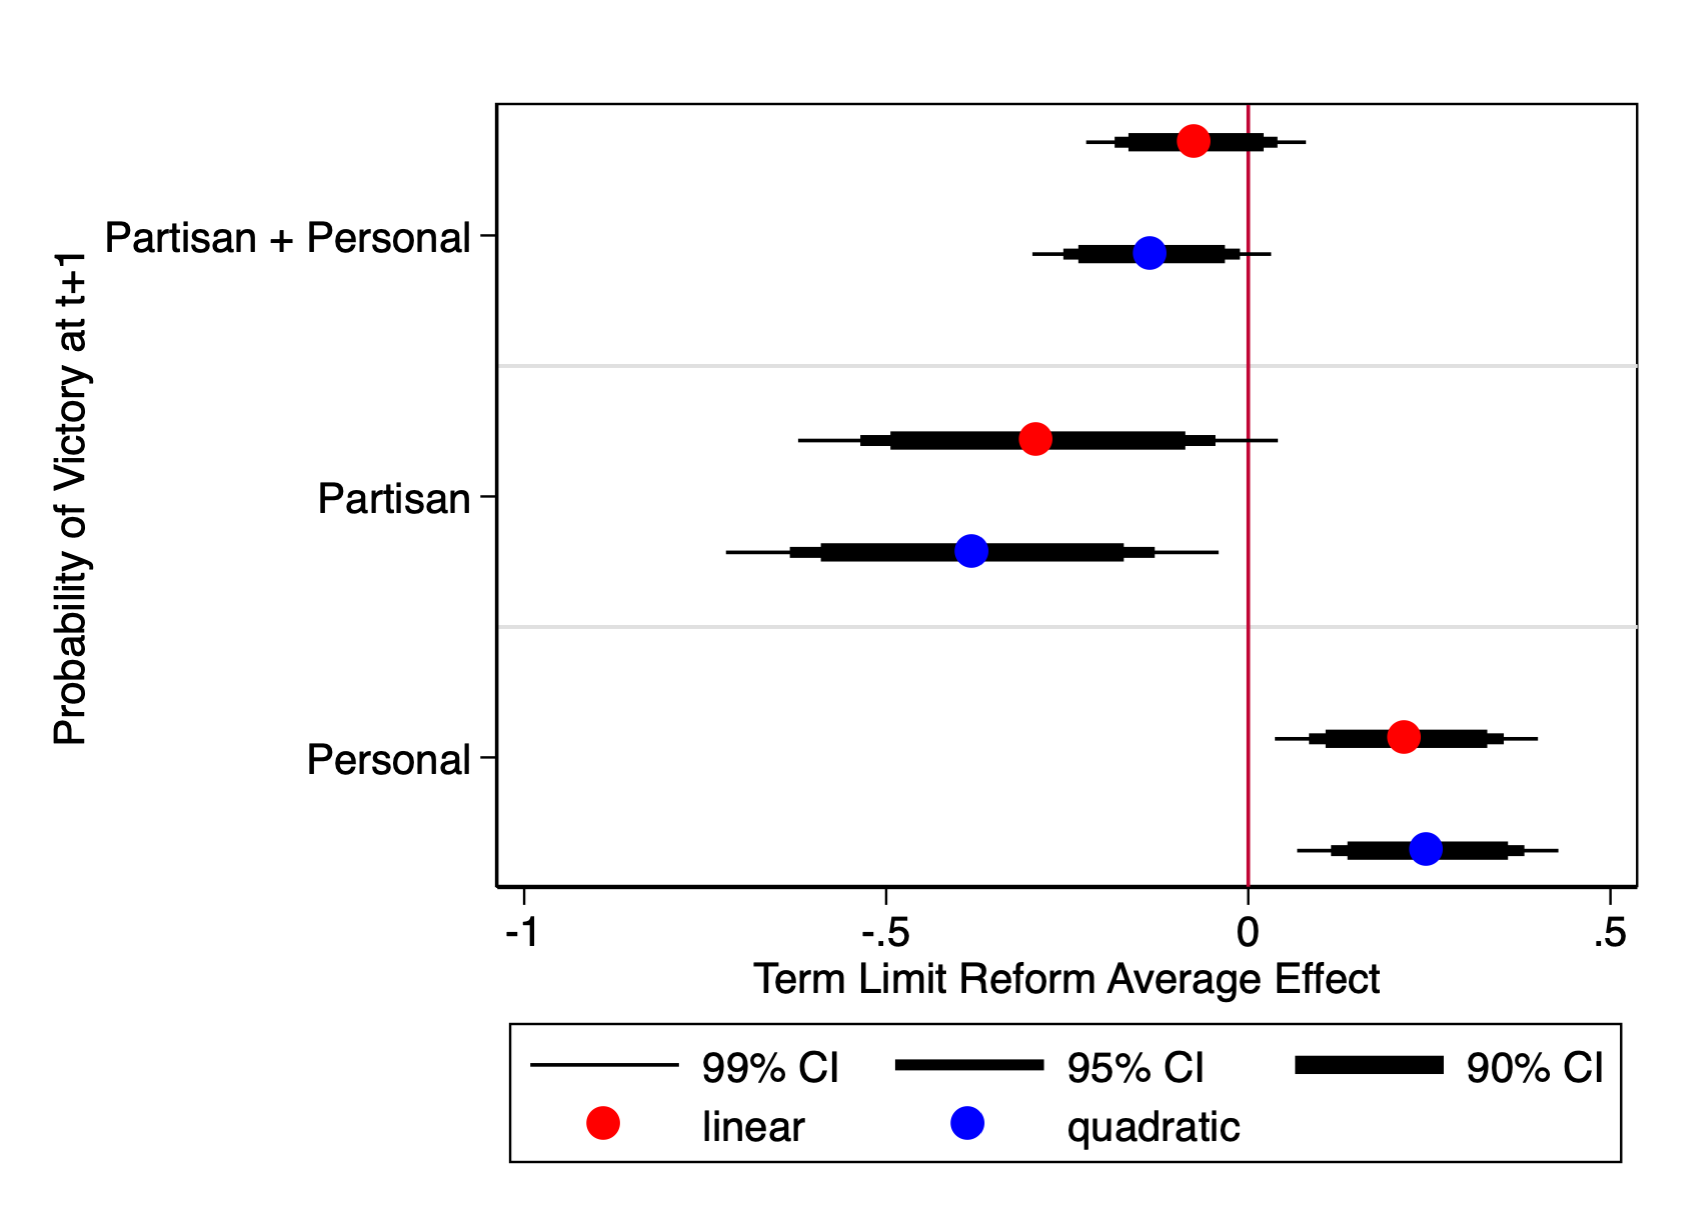
\includegraphics[width=0.9\textwidth]{../Figures_incumbency/partisan_personal_inc_advantage.png}
       \captionsetup{justification=centering}
       
 \textbf{Note:} Figure \ref{fig:personal_vs_partisan} shows the average treatment effect of the Term Limit Reform on the probability of winning in the following election using a difference in discontinuity of close elections design. This average effect was estimated using the IW estimators following \citet{abraham_sun_2020} for each lead and lag relative to the first year a municipality implemented reelection. Optimal bandwidths following \citet{calonicoetal_2014} are used. This analysis identifies the party that wins at $t-1$ and studies the effect of this party barely winning (or losing) at $t$ on outcomes at election $t+1$ following \citet{klasnja_titiunik_2017}. I follow \citet{fowler_hall_2014} to decompose the incumbency advantage into the partisan and personal component. Red and blue points show that parallel trends hold, while hollow ones imply pretrends. 
\end{figure}  

\clearpage

\subsection{Identification assumptions}

To validate causal effects three identification assumptions need to hold. First, cohort weighted specifications need to show parallel trends for both incumbency advantage measures. As seen in Table \ref{tab:incumbency_wpolynomials}  this is the case. Cohort weights further assure that parallel trends are not spurious due to correlation between the $k$ period indicators relative to treatment implementation. Second, no anticipatory behavior from municipalities should be found; since we are only taking into account one election cycle post-treatment, we don't anticipate incumbents reacting in such a short time window. %[MISSING]%this is the case when running an ``event-to-event" analysis following \citet{cengiz_etal_2019}: there is no clustering in estimated coefficients on early and late state adopters.\footnote{Results available upon request.} 
Third, the design would be invalid if parties could manipulate close elections and sort themselves to those that imply a higher probability of winning. Two tests are commonly used to show validity on the design: (a) no covariate jump at the discontinuity on relevant pre-treatment variables and (b) density tests to see whether the number of municipalities above (or below) the cutoff threshold is significantly different from the number of municipalities below (or above). Appendix Figure \ref{tab:incumbency_wpolynomials_pop} showes evidence of no significant jump at the discontinuity of municipal population.\footnote{Next iteration of this working paper will include validation on municipal GDP, revenue and expenditures, geographic location and previous victory.} Furthermore, Appendix Figure \ref{fig:mccrary} shows no density difference between municipalities just above and below the cutoff.\footnote{Given the reduction in sample size from Table \ref{tab:abraham_sun_lagdv} to Table \ref{tab:incumbency_wpolynomials} one could have a concern that main results no longer hold in this close election setting. Appendix Table \ref{tab:abraham_sun_local} shows this is not the case by estimating results of Table \ref{tab:abraham_sun_lagdv} using as sample only the municipalities of the sample of Table \ref{tab:incumbency_wpolynomials}.}   

 \begin{figure}[h]   
\centering
 \caption{Effect of Term Limit Reform on Incumbency Advantage \\ -difference-in-discontinuity of close elections-}
 \label{fig:parallel_trend}
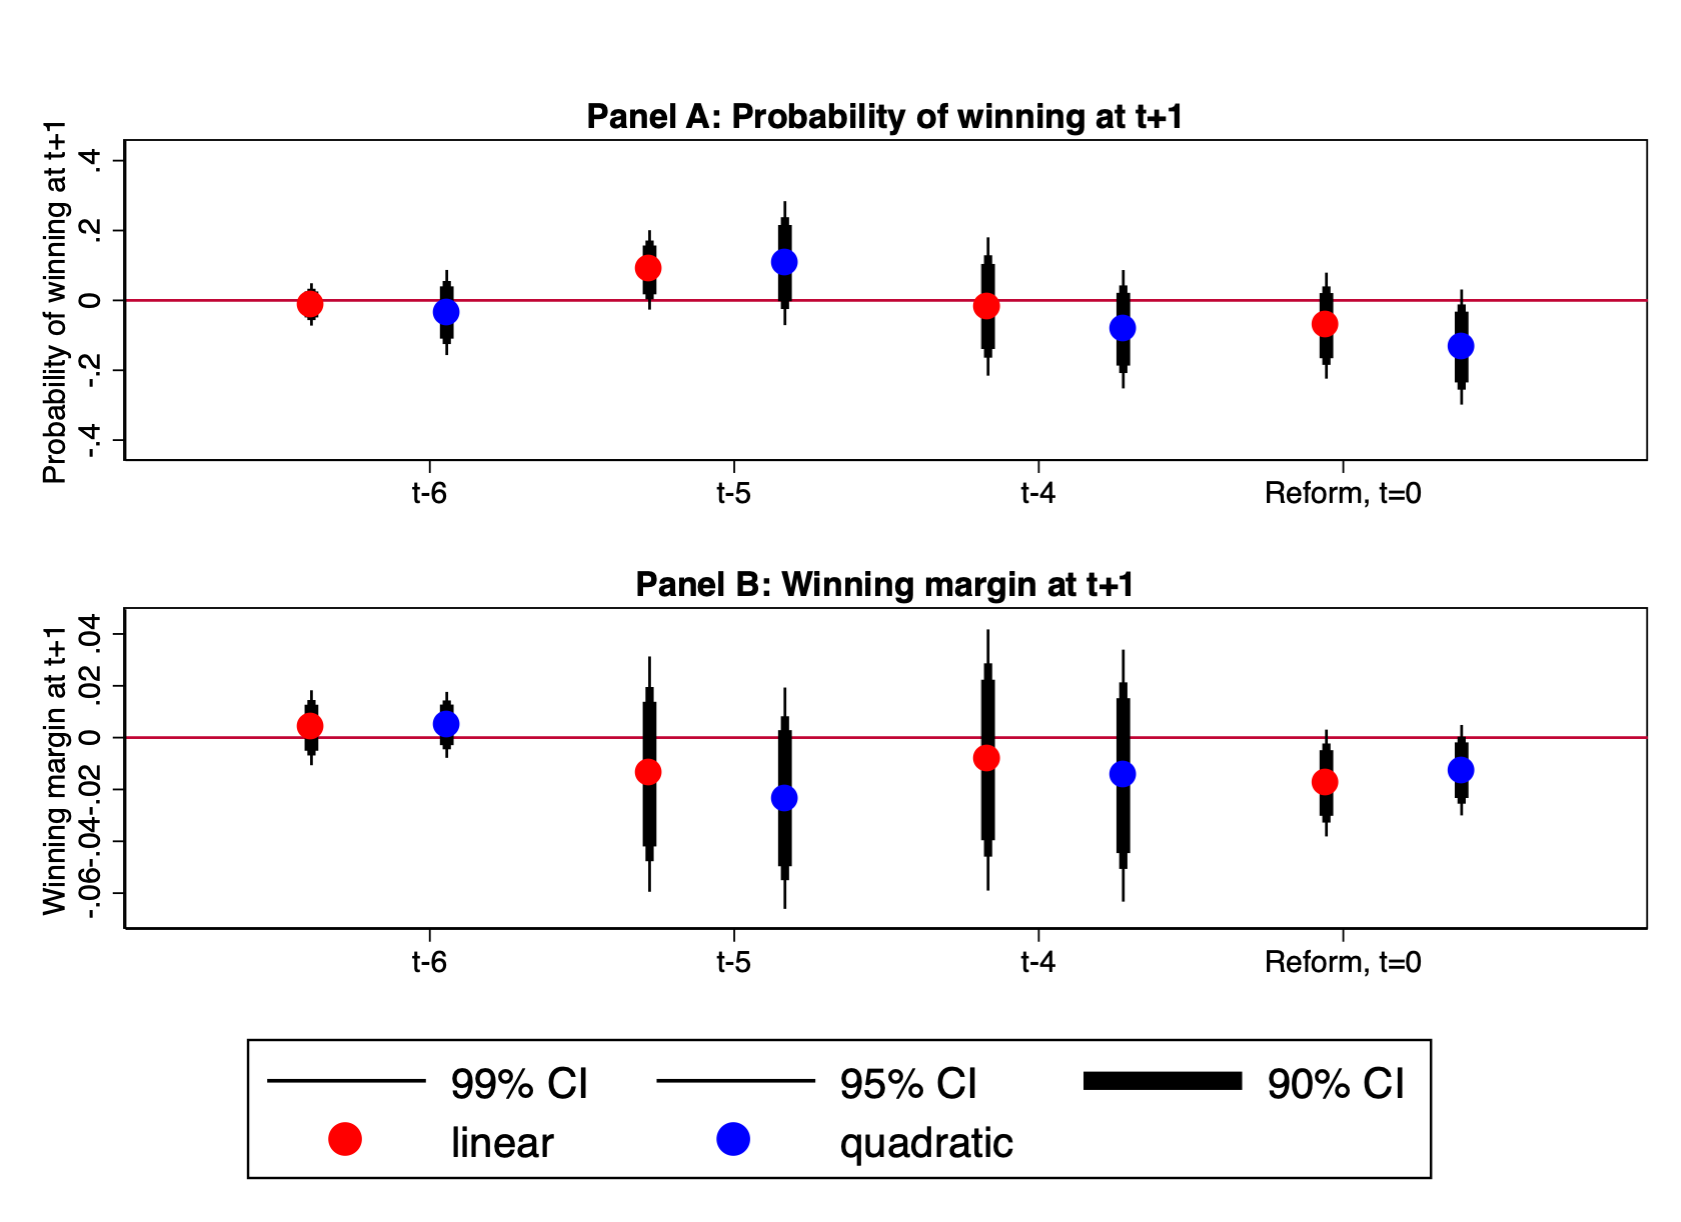
\includegraphics[width=0.9\textwidth]{../Figures_incumbency/parallel_trend.png}
       \captionsetup{justification=centering}
         
 \textbf{Note:} Figure \ref{fig:parallel_trend} shows the average treatment effect of the Term Limit Reform on the probability of winning in the following election using a difference in discontinuity of close elections design. This average effect was estimated using the IW estimators following \citet{abraham_sun_2020} for each lead and lag relative to the first year a municipality implemented reelection. Optimal bandwidths following \citet{calonicoetal_2014} are used. This analysis identifies the party that wins at $t-1$ and studies the effect of this party barely winning (or losing) at $t$ on outcomes at election $t+1$ following \citet{klasnja_titiunik_2017}.  
 
\end{figure}   

Overall, results show the Term Limit Removal Reform increased incumbent probability of winning at future elections. If this is the case, then we should expect a decrease in the effort placed by security forces in the country, especially from the party in government, the PRI. Federal forces, particularly the military in charge of tackling DTOs, should decrease the amount of narcotic crackdowns and seizures. Furthermore, this should generate a downward effect to local proxies, i.e. mayors in charge of tackling down local crime. In fact, this is what I find. 
   \clearpage
  
\section{Robustness}
      
 Results are robust to controlling for incumbent quality.\footnote{Results available upon request.} 
\begin{table}[htbp]\def\sym#1{\ifmmode^{#1}\else\(^{#1}\)\fi}
\centering
\caption{Personal and Partisan Incumbency Advantage following \citet{fowler_hall_2014}}
\label{tab:fowler_hall}
\scalebox{1}{
\begin{tabular}{lccc}
\hline \hline
& \multicolumn{3}{c}{\textbf{Panel A: linear polynomial}}\\
& \multicolumn{1}{c}{No term limits:} & \multicolumn{1}{c}{term limits:} & \multicolumn{1}{c}{difference:}\\
Advantage: & \multicolumn{1}{c}{personal + partisan} & \multicolumn{1}{c}{partisan} & \multicolumn{1}{c}{personal} \\
& \multicolumn{1}{c}{(1)} & \multicolumn{1}{c}{(2)} & \multicolumn{1}{c}{(3)} \\
\cmidrule(lrr){2-2}  \cmidrule(lrr){3-3} \cmidrule(lrr){4-4}\\
\addlinespace
RD estimate: prob(victory in t+1) &      $ 0.0568^{} $ &  $ -0.1269^{***} $  &  $ 0.1468^{***} $  \\
& ($ 0.0508$) & ($ 0.0208 $)  & ($ 0.0038 $)\\
RD estimate: vote share in t+1 &      $ 0.0245^{} $ &  $ -0.0529^{***} $  &  $ 0.0618^{***} $  \\
& ($ 0.0243$) & ($ 0.0073 $)  & ($ 0.0024 $)\\
\addlinespace
Observations: prob(victory in t+1)      &            1257        &     9180  \\
Observations: vote share in t+1      &            1221        &     8758  \\
\\
& \multicolumn{3}{c}{\textbf{Panel B: quadratic polynomial}}\\
& \multicolumn{1}{c}{No term limits:} & \multicolumn{1}{c}{term limits:} & \multicolumn{1}{c}{difference:}\\
Advantage: & \multicolumn{1}{c}{personal + partisan} & \multicolumn{1}{c}{partisan} & \multicolumn{1}{c}{personal} \\
& \multicolumn{1}{c}{(1)} & \multicolumn{1}{c}{(2)} & \multicolumn{1}{c}{(3)} \\
\cmidrule(lrr){2-2}  \cmidrule(lrr){3-3} \cmidrule(lrr){4-4}\\
\addlinespace
RD estimate: prob(victory in t+1) &      $ 0.0442^{} $ &  $ -0.1291^{***} $  &  $ 0.1384^{***} $  \\
& ($ 0.0676$) & ($ 0.0258 $)  & ($ 0.0042 $)\\
RD estimate: vote share in t+1 &      $ 0.0311^{} $ &  $ -0.0510^{***} $  &  $ 0.0656^{***} $  \\
& ($ 0.0274$) & ($ 0.0092 $)  & ($ 0.0026 $)\\
\addlinespace
Observations: prob(victory in t+1)      &            1257        &     9180  \\
Observations: vote share in t+1      &            1221        &     8758  \\
\hline \hline
\multicolumn{4}{p{1\textwidth}}{\footnotesize{Notes: Standard errors in parentheses are clustered at the state level, with the following significance-level: $^{***}$ 1\%; $^{**}$ 5\%; and $^*$ 10\%, that refer to two-sided t-test with the null hypothesis equal to 0 for each relative time period. Table estimated using all elections since the year 2000.}}
\end{tabular}
}
\end{table}
   

%Talk about testing different bandwidths 

\clearpage

\section{Mechanisms}

Over the past decades, an important theoretical and empirical literature in American Politics has shown that incumbents enjoy an electoral advantage. A big concern faced by the literature has been understanding the determinants of incumbency advantage. To date, we can identify at least three types of explanations.  First, what incumbents do (and opponents cannot do) emphasizing the resources, visibility, and power that incumbents gain from office holding (Mayhew 1974; Fiorina 1977, 1989; King 1991; Cox and Morgenstern 1993). Second, quality-based explanations that emphasize who incumbents are (and who their opponents are) (Cox and Katz, 1996; Levitt and Wolfram, 1997; Ansolabehere and Snyder, 2002) [for a discussion of these two types of mechanisms, please see Eggers (2017)]. In this second line we find explanations related to incumbents’ quality as well as the “scare-off effect”, or the ability incumbents have to scare off high-quality challengers. A third and more recent type of mechanism emphasizes the role of information. Ashworth and Bueno de Mesquita (2008) find that incumbency advantage is dependent on how precise the information is about incumbent’s ability to voters. More recently, Ashworth, Bueno de Mesquita and Friedenberg (2019) expand on the role of information to explain incumbency advantage: through a theoretical model, they show that incumbents have an additional information advantage to challengers: they govern while challengers do not. This is so even absent any partisanship, electoral selection or challenger scare off. However, to date there is no empirical identification of the information-based explanation proposed by these authors. Moreover, if theoretical work done by Ashworth and co-authors is correct, all other explanations of incumbency advantage might be biased by the role information plays. 

 \begin{figure}[h]   
\centering
 \caption{Effect of Term Limit Reform on the Quality of Candidates}
 \label{fig:quality_trend}
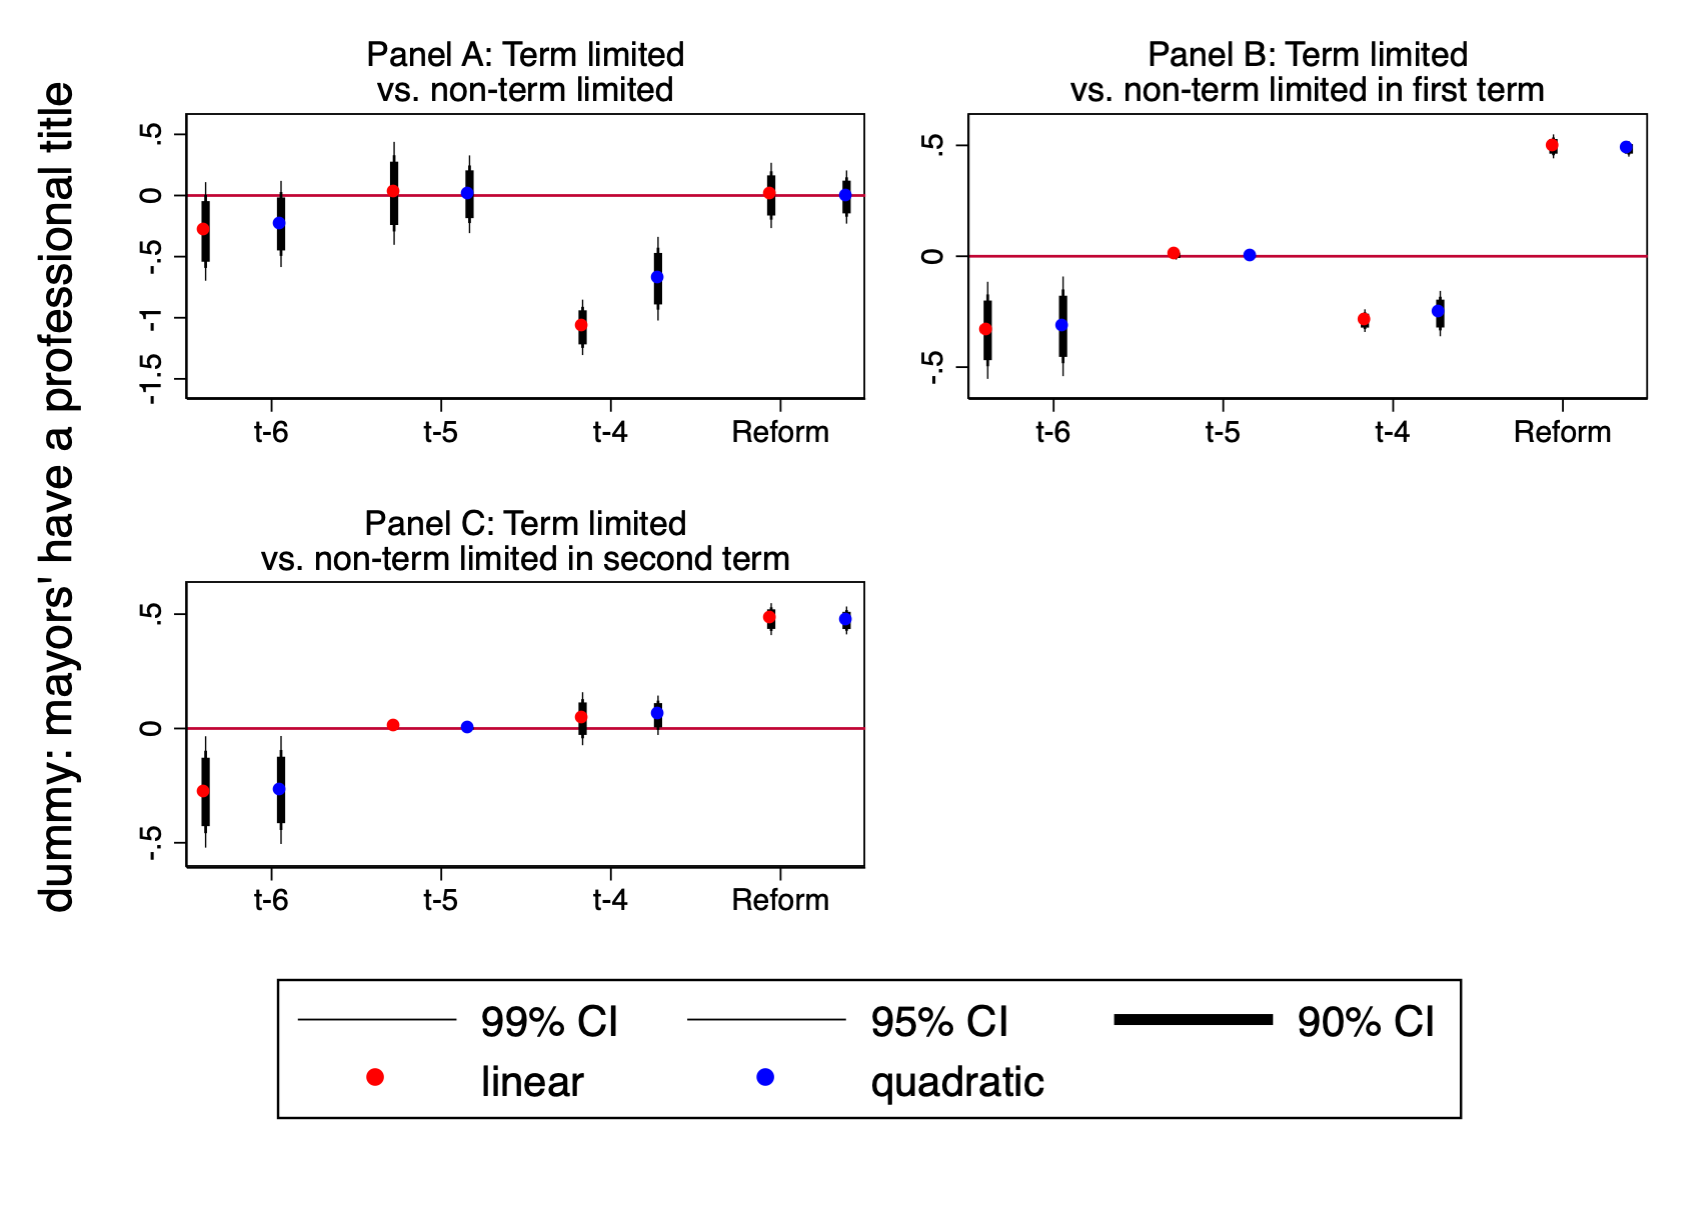
\includegraphics[width=0.9\textwidth]{../Figures_incumbency/quality_parallel.png}
       \captionsetup{justification=centering}
         
 \textbf{Note:} Figure \ref{fig:quality_trend} shows the average treatment effect of the Term Limit Reform on a dummy indicator of whether candidates hold a professional title. This average effect was estimated using the IW estimators following \citet{abraham_sun_2020} for each lead and lag relative to the first year a municipality implemented reelection. Same optimal bandwidths as those in Figure \ref{fig:parallel_trend} are used, as well as the same number of observations.  
 
\end{figure}     

  
	
\begin{figure}[h]   
\centering
 \caption{Effect of Term Limit Reform on Municipal Revenues}
 \label{fig:revenues1}
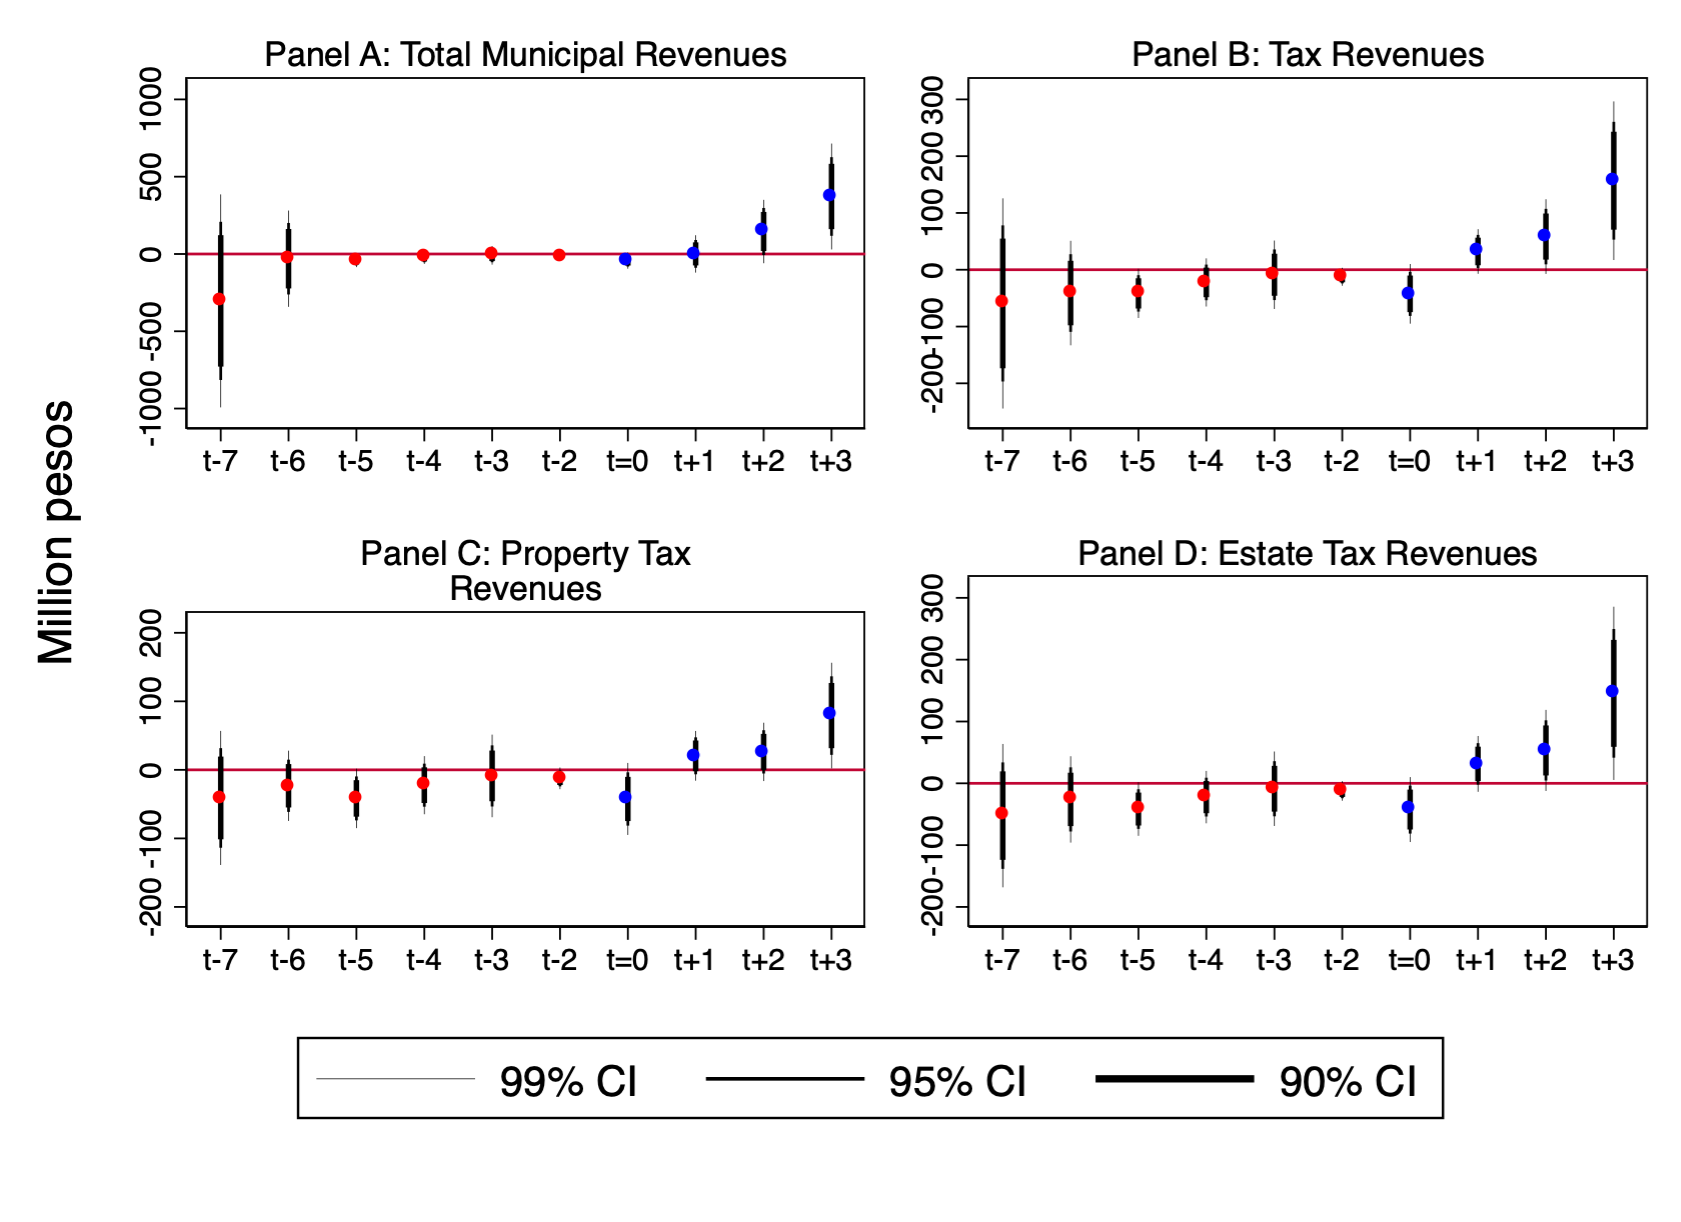
\includegraphics[width=0.9\textwidth]{../Figures/revenues_allyears1.png}
       \captionsetup{justification=centering}
         
 \textbf{Note:} Figure \ref{fig:revenues1} shows the average treatment effect of the Term Limit Reform on a dummy indicator of whether candidates hold a professional title. This average effect was estimated using the IW estimators following \citet{abraham_sun_2020} for each lead and lag relative to the first year a municipality implemented reelection. Same optimal bandwidths as those in Figure \ref{fig:parallel_trend} are used, as well as the same number of observations.  
       
\end{figure}   

\begin{figure}[h]   
\centering
 \caption{Effect of Term Limit Reform on Municipal Revenues (continuation)}
 \label{fig:revenues2}
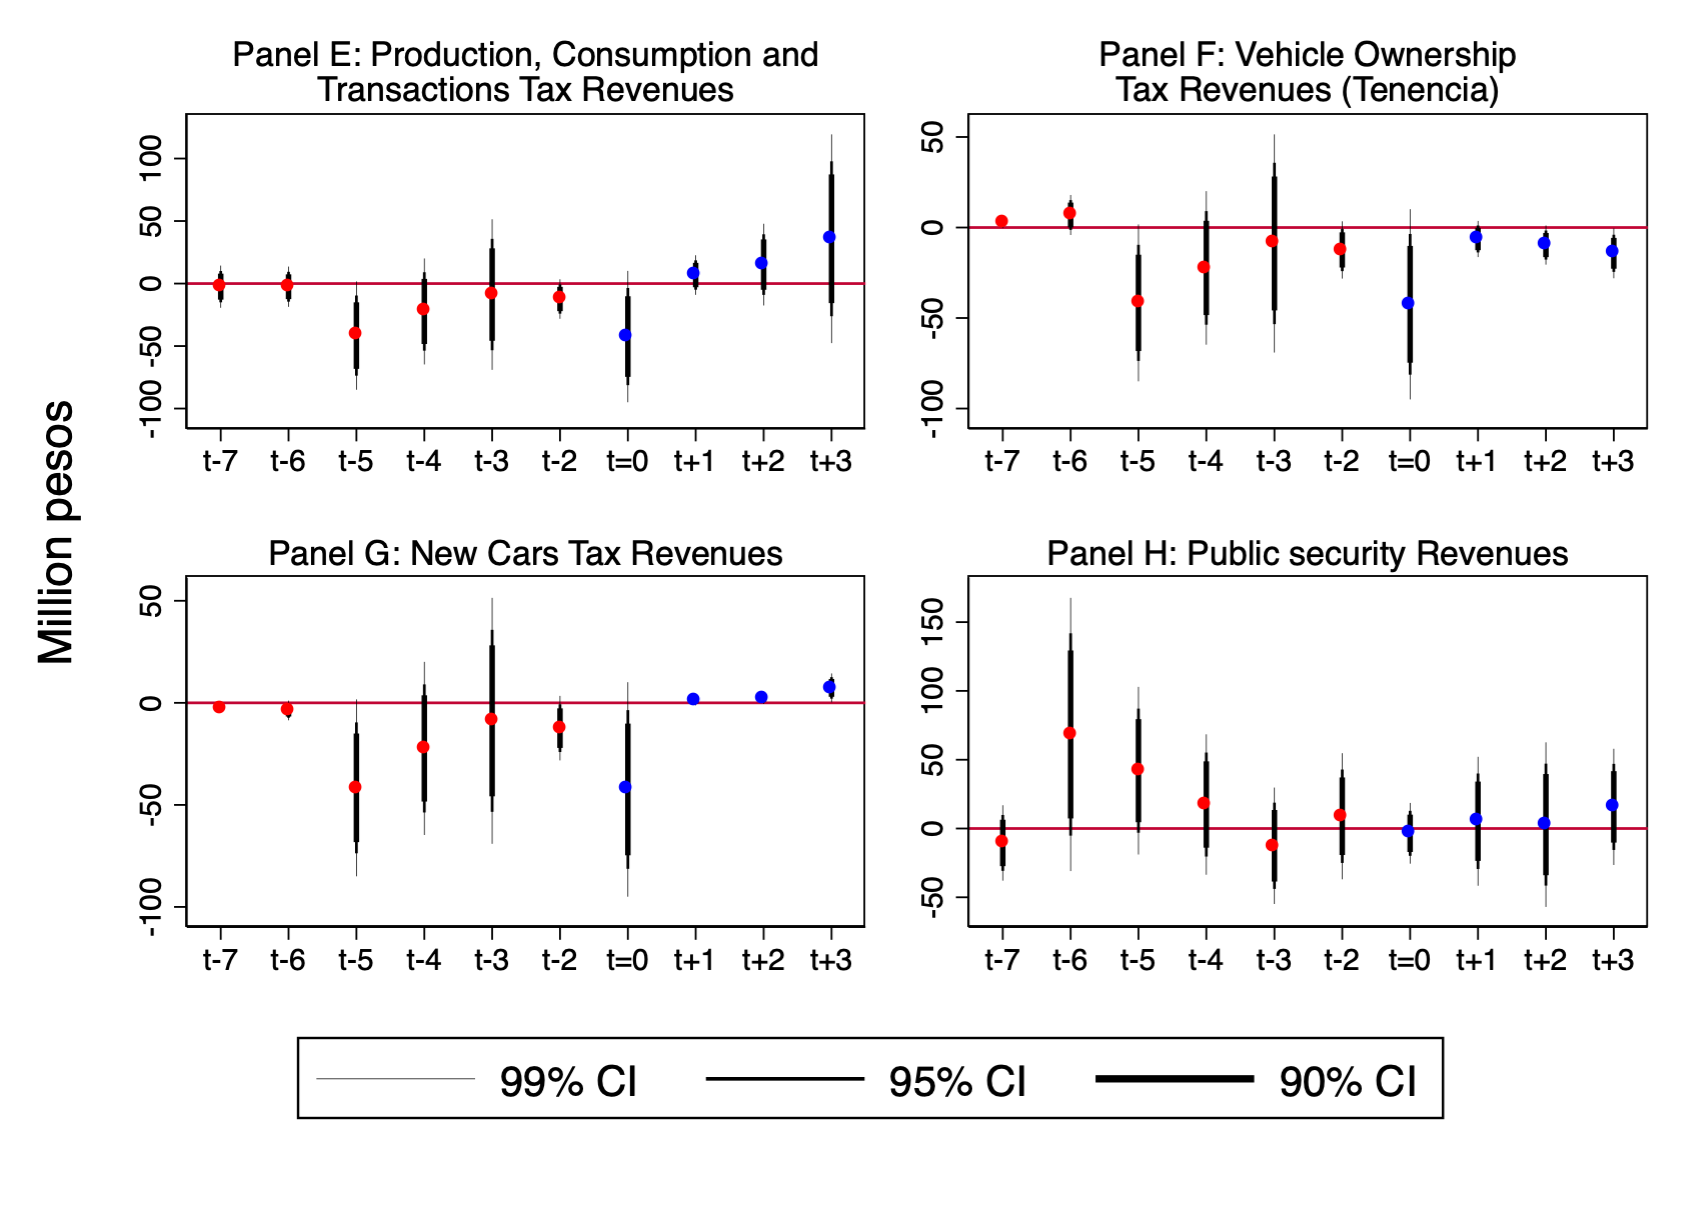
\includegraphics[width=0.9\textwidth]{../Figures/revenues_allyears2.png}
       \captionsetup{justification=centering}
         
 \textbf{Note:} Figure \ref{fig:revenues2} shows the average treatment effect of the Term Limit Reform on a dummy indicator of whether candidates hold a professional title. This average effect was estimated using the IW estimators following \citet{abraham_sun_2020} for each lead and lag relative to the first year a municipality implemented reelection. Same optimal bandwidths as those in Figure \ref{fig:parallel_trend} are used, as well as the same number of observations.  
          
\end{figure}     

\begin{figure}[h]   
\centering
 \caption{Effect of Term Limit Reform on Transfers from the Federation or the State}
 \label{fig:resources2}
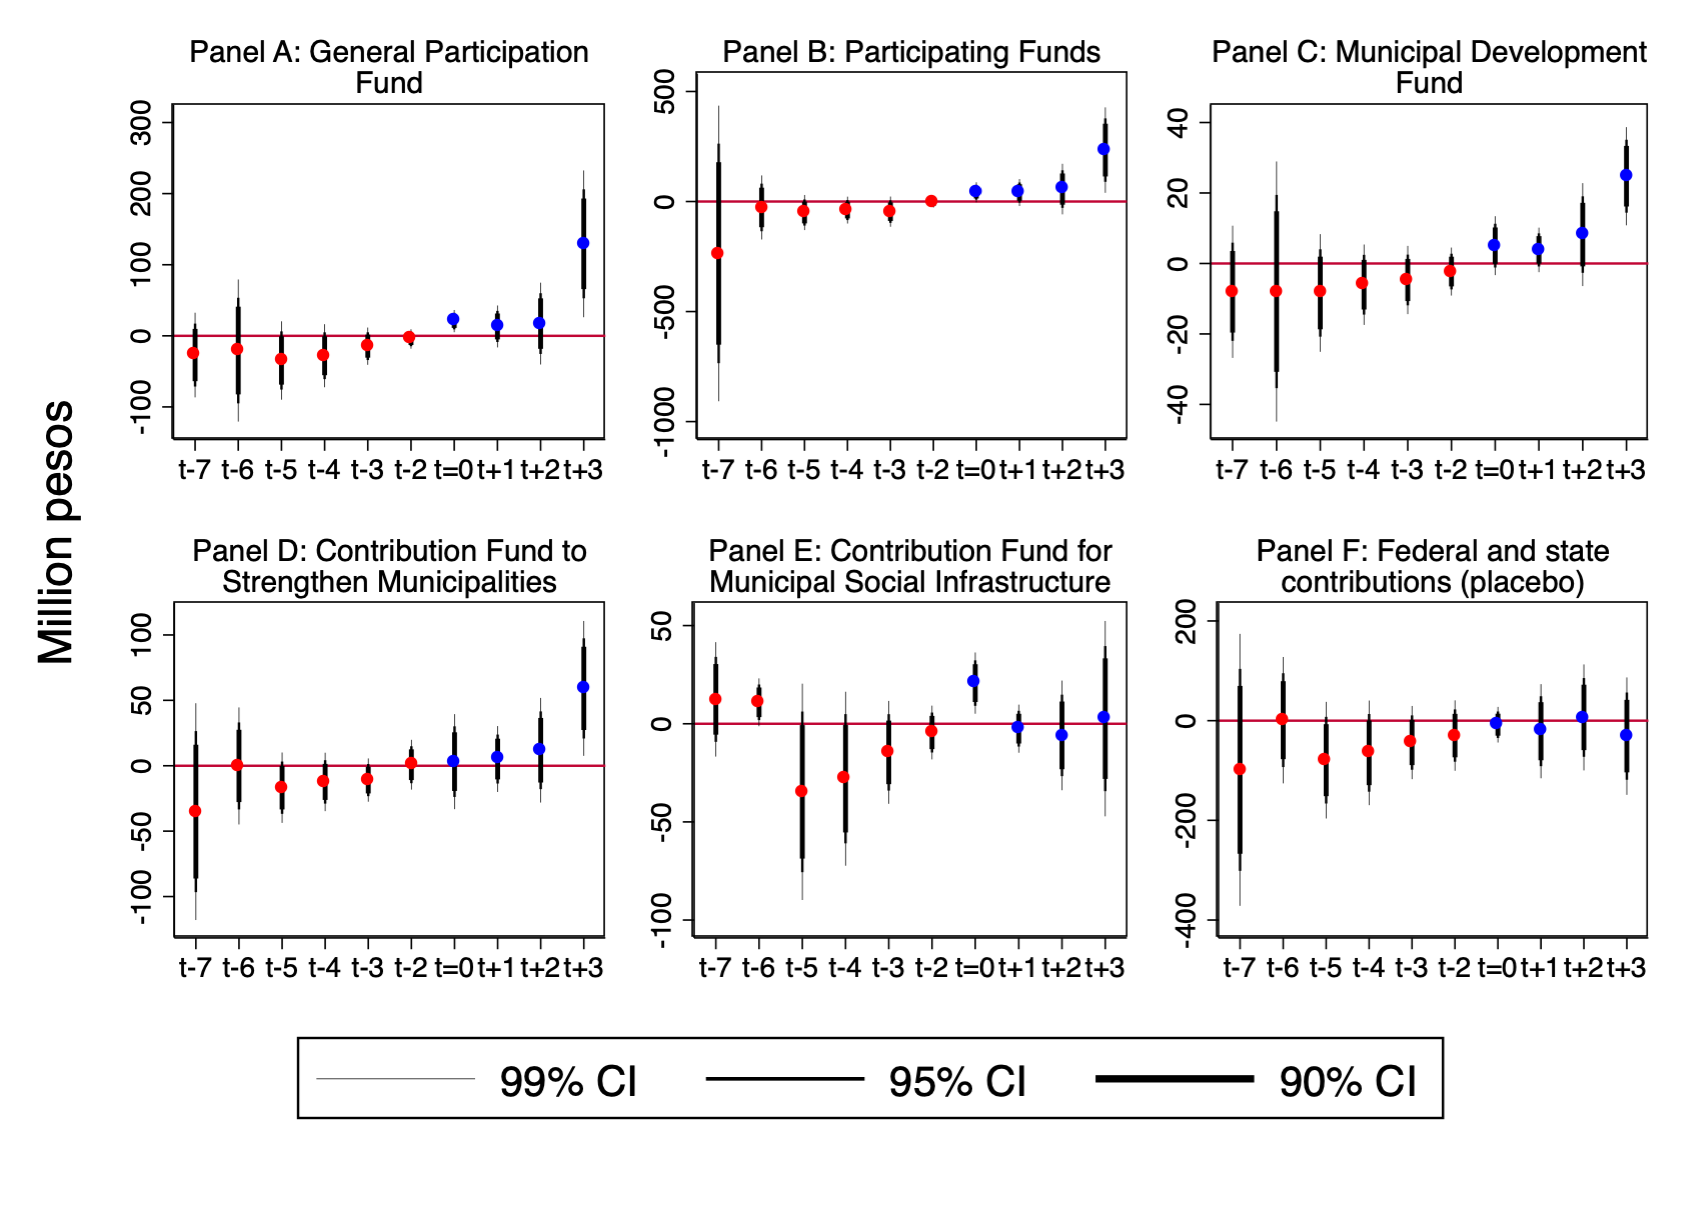
\includegraphics[width=0.9\textwidth]{../Figures/resouce_based_incumbency_allyears.png}
       \captionsetup{justification=centering}
         
 \textbf{Note:} Figure \ref{fig:resources2} shows the average treatment effect of the Term Limit Reform on a dummy indicator of whether candidates hold a professional title. This average effect was estimated using the IW estimators following \citet{abraham_sun_2020} for each lead and lag relative to the first year a municipality implemented reelection. Same optimal bandwidths as those in Figure \ref{fig:parallel_trend} are used, as well as the same number of observations.  
       
\end{figure}  

 \begin{figure}[h]   
\centering
 \caption{Effect of Term Limit Reform on the Effort of Incumbents}
 \label{fig:effort}
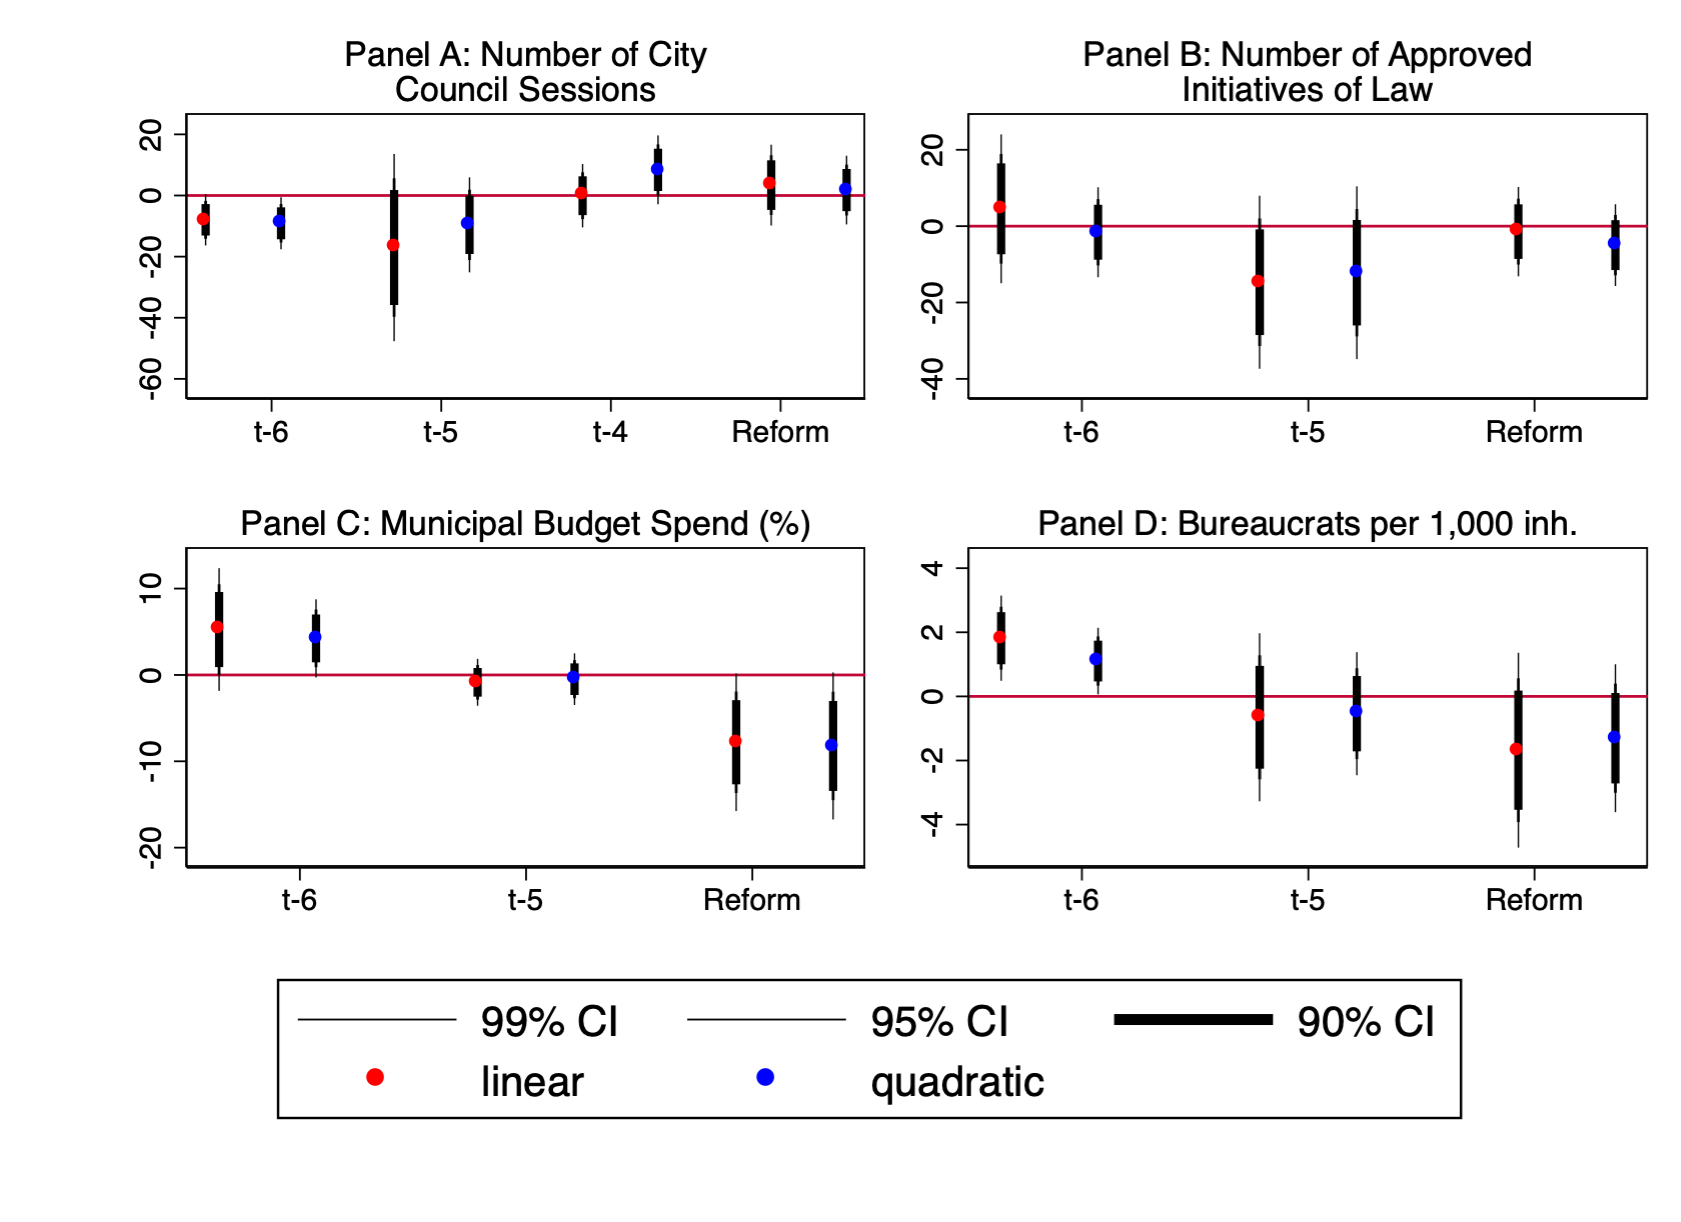
\includegraphics[width=0.9\textwidth]{../Figures_incumbency/effort_based_incumbency.png}
       \captionsetup{justification=centering}
         
 \textbf{Note:} Figure \ref{fig:effort} shows the average treatment effect of the Term Limit Reform on a dummy indicator of whether candidates hold a professional title. This average effect was estimated using the IW estimators following \citet{abraham_sun_2020} for each lead and lag relative to the first year a municipality implemented reelection. Same optimal bandwidths as those in Figure \ref{fig:parallel_trend} are used, as well as the same number of observations.  
 
\end{figure}    
   
 \begin{figure}[h]   
\centering
 \caption{Effect of Term Limit Reform on Municipal Expenses}
 \label{fig:expenses}
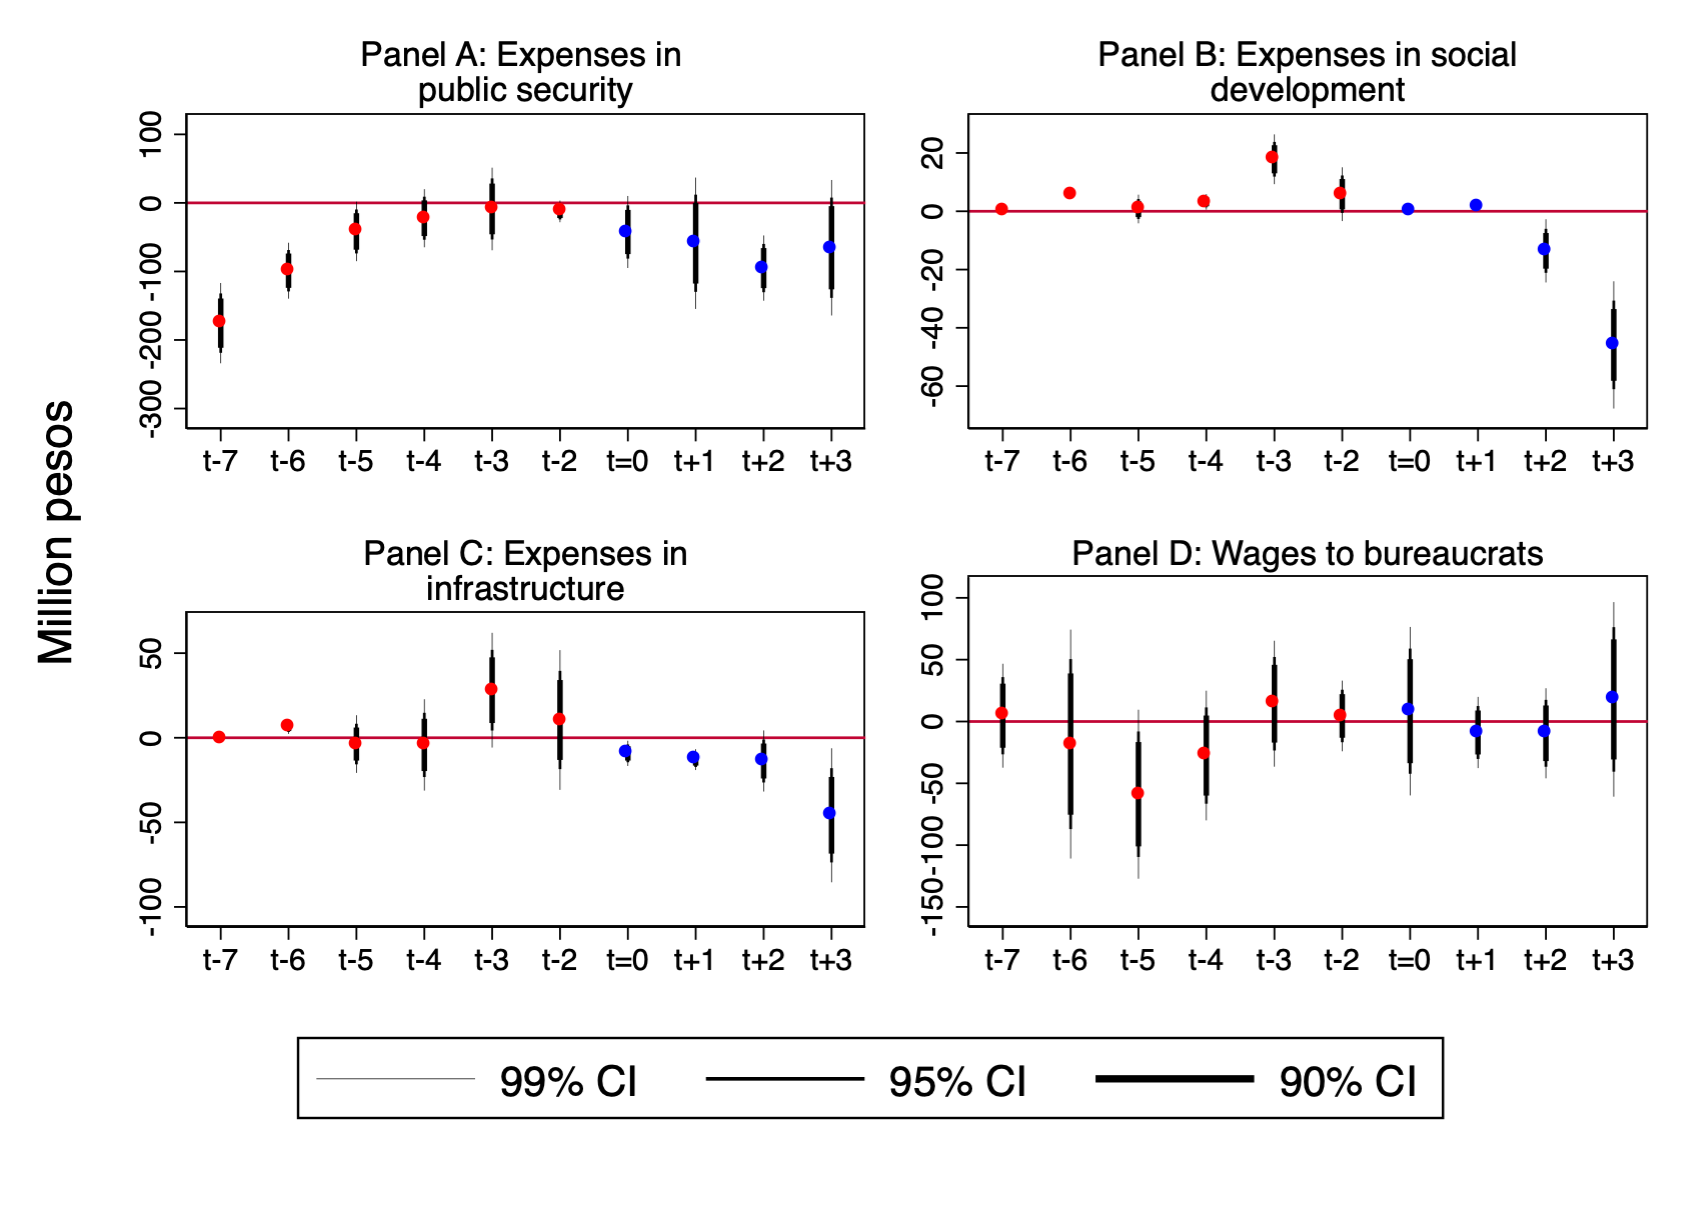
\includegraphics[width=0.9\textwidth]{../Figures/expenses_allyears.png}
       \captionsetup{justification=centering}
         
 \textbf{Note:} Figure \ref{fig:expenses} shows the average treatment effect of the Term Limit Reform on a dummy indicator of whether candidates hold a professional title. This average effect was estimated using the IW estimators following \citet{abraham_sun_2020} for each lead and lag relative to the first year a municipality implemented reelection. Same optimal bandwidths as those in Figure \ref{fig:parallel_trend} are used, as well as the same number of observations.  
     
\end{figure}    

                      
\clearpage
\section{Discussion on Parties-Members Relations with Asymmetric Personal and Partisan Incumbency Returns}


A positive return to incumbency:
The typical finding is that incumbents outperform non-incumbents \citep{gelman_king_1990, cox_morgensten_1993, ansolabehere_snyder_2000, hirano_snyder_2009}. This can be due to...
\begin{itemize}
	\item Parties shape policy \citep{cox_mccubins_1993, cox_mccubins_2006}, and policy generates electoral returns (cite from reelection backfire) 
	\item they draw loyalty from voters \citep{campbell_etal_1960, green_etal_2002}. 
	\item sophomore surge: new official will garner more votes when running for his first reelection than when she was a challenger \citep{erikson_1971, alford_brady_1989}.
\end{itemize}

But an incumbency disadvantage can also be present: 
\begin{itemize}
	\item voters prefer partisan balance \citep{campbell_miller_1957, lewis_beck_2004, folke_snyder_2012}
	\item voters dislike political institutions relative to incumbent officials \citep{fenno_1975, parker_davidson_1979}. 
	\item grass-is-greener effect and value outside options, even when the candidate is from a bad type \citep{brenner_etal_2007, bordalo_etal_2012, bhaia_turan_2013}
	\item \citep{klasnja_titiunik_2017} explanation
	\item retirement slump: parties lose votes when the incumbent retires \citep{alford_brady_1989}, or when there are term limits \citep{ansolabehere_snyder_2004}. 
	\item Institutional changes, including redistricting, may decrease electoral support of incumbents \citep{ansolabehere_etal_2000, desposato_petrocik_2003} 

\end{itemize} 

if voters perceive incumbents are captured, information from the first period in office may not be enough to determine the performance of a second term in office. The result is incumbency disadvantage \citep{weaver_2020}.

Reasons behind incumbency advantage (similar to the introduction of fowler and hall 2014). 

For voters, reelection increases political accountability: it creates an instrument for constituents to punish bad behaviors from  representatives and reward good ones, a bottom-up accountability \citep{mansbridge_2009}. Information for casting a vote is key: if current performance can predict future performance then voters can assess incumbents and choose to reelect them or not \citep{ashworth_2012}.  

There are cases, however, where information of performance in office is not enough for voters to assess if good performance will continue if an incumbent is elected again. Three features, at least, constraint voter information. First, the notion that incumbents experience is correlated not only with good performance in terms of public good provision and desired policies, but also with corruption: a term in office allows politicians to learn how to provide a public good and approach voters, as well as detect malfeasance and economic opportunities (and networks) for personal gain. \citet{coviello_etal_2017} find that terms in office leads politicians to identify local bidders, reduce the number of bidders per auction, increase the cost of procurement and a decrease in competition (fewer firms winning auctions). \citet{fisman_etal_2014} find that, for the case of India for example, incumbents' assets grow 3-4\% faster than those of second runners, something slightly higher for incumbents who won in close elections, and gain tied to secondary corruption activities. Political experience can also be tied with clientelistic practices: a term in office allows politicians to better understand, detect and capture clienteles, reducing their electoral accountability to the median voter (cite here). Likewise, a term in office may lead to collusion between local executives and DTOs. Overall, as a result of the corruption or collusion perceived by voters, they may prefer to vote for a new pool of candidates generating an incumbency \emph{disadvantage} (e.g. \citet{klasnja_2015} in Romania; for an overview see \citet{klasnja_2016}). An incumbency disadvantage decreases politicians' incentive to cater to the median voter and choose to focus on particularistic spending. %(cite here). 

A second reason that makes voters disregard information from an incumbent's first term in office is weak oversight of politicians.\footnote{Other reasons that may affect reelection as an instrument for political accountability are voter bias or being unable to process performance information correctly \citep{dunning_etal_2019, bhandari_etal_2019}, incumbent misalignment with median voters needs (see \citet{adida_etal_2017}, \citet{boas_etal_2019} or \citet{dekadt_etal_2017} for examples) or not assessing blame to local executives for the provision of a specific public good (e.g. mayors are blamed for public water provision but not security). While relevant, I do not delve into these reasons as voter information processing is not the main objective of this paper. Additionally, an event-study design allows me to have a treatment and control group that, on average, should have equal amount of voters wrongly processing incumbents performance in office, as well as mismatch between incumbents policies and those desired by voters or constituents that assess credit-blame similarly.} \citet{weaver_2020} notes that \emph{horizontal} accountability is key for reelection to generate political accountability:\footnote{We know that horizontal accountability institutions have led to political accountability. \citet{hidalgo_etal_2015} finds that Brazilian voter audits or electoral revisions in charge of detecting fraudulent registration curbed voter buying. Meanwhile, \citet{fujiwara_2015} finds that the introduction of electronic voting in Brazil increased public good provision of goods particularly relevant to those that got enfranchised, the poor.} if institutions such as the judiciary, and audit offices are not able to enforce politicians behavior, politicians may misbehave in office in their second term, making performance in office from the first term insufficient information for voters to cast a vote. As a result, incumbency disadvantage may also result from weak horizontal accountability (or vertical, like that of parties). 


On the contrary, a party-level incumbency \emph{advantage}, implies that information of a first term in office yields relevant information for constituents to assess a politicians' performance \citep{weaver_2020}. Given the discussion above, this happens because (a) voters do not associate a first term with experience on corruption or collusion, and (b) they believe strong horizontal and vertical accountability institutions are set in place to oversight incumbents behavior. Formally, we can derive the following hypothesis:
 

\bigskip

\textbf{H4:} An incumbency advantage shows that information of an incumbent first term in office yields sufficient information for voters to assess incumbent's performance. 
\\
 
Importantly, while voters may identify strong vertical accountability institutions, such as parties, they may not notice the willingness parties may have to monitor. Taking hypotheses \textbf{H1} and \textbf{H4}, we find an accountability paradox: parties strong capacity to oversight may lead voters to create an incumbency advantage in the presence of reelection, while an incumbency advantage decreases the willingness of parties to do so.  

 %This incumbency advantage further reflects information not only on politicians, but also on parties \citep{fowler_hall_2014, erikson_titiunik_2015}.%check this last statement. This is very important. If there is no information problem, then its all about monitoring.  


\clearpage
                  

\section{Conclusion} 

               
%APPENDIX -----------------------------------------------

%%%%%%%%%%%%
\bibliographystyle{aer} 
\bibliography{References}    

\clearpage
%APPENDIX -----------------------------------------------
\begin{appendix}

%%%%%%%%%%%%%%%%%%%%%%%%%%%%%%%%% 

\section{Tables and Figures \label{appendix:tables_figures}}
 
\renewcommand{\thetable}{A-\arabic{table}}
\setcounter{table}{0}
 
\renewcommand{\thefigure}{A-\arabic{figure}}
\setcounter{figure}{0}
   
\begin{table}[htbp]\def\sym#1{\ifmmode^{#1}\else\(^{#1}\)\fi}
\centering
\caption{Difference-in-Discontinuity in close elections model: Effect of 2014 Term Limit Reform on Incumbency Advantage}
\label{tab:incumbency_wpolynomials}
\scalebox{0.8}{
\begin{tabular}{lcc}
\hline \hline
\\ \multicolumn{3}{l}{Dependent variable:}\\
& \multicolumn{1}{c}{Probabilitiy of winning at t+1}  & \multicolumn{1}{c}{Winning margin at t+1} \\
& \multicolumn{1}{c}{(indicator)}  & \multicolumn{1}{c}{(indicator)} \\
& \multicolumn{1}{c}{(1)} & \multicolumn{1}{c}{(2)}  \\
\cmidrule(lrr){2-2}  \cmidrule(lrr){3-3} \\
\addlinespace
& \multicolumn{2}{c}{linear polynomial} \\
\cmidrule(lrr){2-3} \\
t-6 &       $ -0.0116^{} $ &       $ 0.0038^{} $  \\
& ($ 0.0219 $ ) & ($ 0.0052 $ ) \\
t-5 &       $ 0.0872^{**} $ &        $ -0.0141^{} $ \\
& ($ 0.0410 $ ) & ($ 0.0164 $ ) \\
t-4 &          $ -0.0175^{} $ &       $ -0.0086^{} $ \\
& ($ 0.0715 $ ) & ($ 0.0182 $ ) \\
Election after Reform &         $ -0.0723^{} $ &        $ -0.0175^{**} $ \\
& ($ 0.0547 $ ) & ($ 0.0074 $ ) \\
Observations          &              2,071     &              6,897 \\
R-squared        &          0.5528   &          0.7105 \\
\\
& \multicolumn{2}{c}{quadratic polynomial} \\
\cmidrule(lrr){2-3} \\
t-6 &       $ -0.0347^{} $ &       $ 0.0049^{} $  \\
& ($ 0.0440 $ ) & ($ 0.0046 $ ) \\
t-5 &       $ 0.1066^{} $ &        $ -0.0234^{} $ \\
& ($ 0.0641 $ ) & ($ 0.0154 $ ) \\
t-4 &          $ -0.0826^{} $ &       $ -0.0147^{} $ \\
& ($ 0.0611 $ ) & ($ 0.0175 $ ) \\
Reform, t=0 &         $ -0.1335^{**} $ &        $ -0.0126^{*} $ \\
& ($ 0.0595 $ ) & ($ 0.0063 $ ) \\
Observations          &              2,845     &              2,845 \\
R-squared        &          0.5445   &          0.6365 \\
\\
Mun. FEs        &     \checkmark         &  \checkmark   \\
Year. FEs     &     \checkmark         &  \checkmark  \\
Controls$^a$  &    \checkmark     &       \checkmark \\
Cohort weighted  &         \checkmark &         \checkmark \\
\hline \hline
\multicolumn{3}{p{0.9\textwidth}}{\footnotesize{Notes: Coefficients show IW estimators following \citet{abraham_sun_2020}. Two relative time periods (lag 8 and 3) are removed to avoid collinearity problems noted by \citet{abraham_sun_2020} or because they are collinear or inexistent, like lag time period 1 and 2. The reference period is t-3, i.e. the municipal elections that ocurred 3 years prior to the reform. Standard errors in parentheses are clustered at the state level for estimates in saturaded model. Significance-level: $^{***}$ 1\%; $^{**}$ 5\%; and $^*$ 10\%, that refer to two-sided t-test with the null hypothesis equal to 0 for each relative time period.$^a$ Pretreatment controls include: governor winning margin; party alignment with the President;  party alignment with the Governor; municipal winning margin; and logged population.}} \\
\end{tabular}
}
\end{table}
   
         

%Figure:  
\begin{comment}
	
 \begin{figure}[H]   
\centering
 \caption{Personal and Partisan Incumbency Advantage, two-way fixed effect model}
 \label{fig:twfe_partisan&personal}
 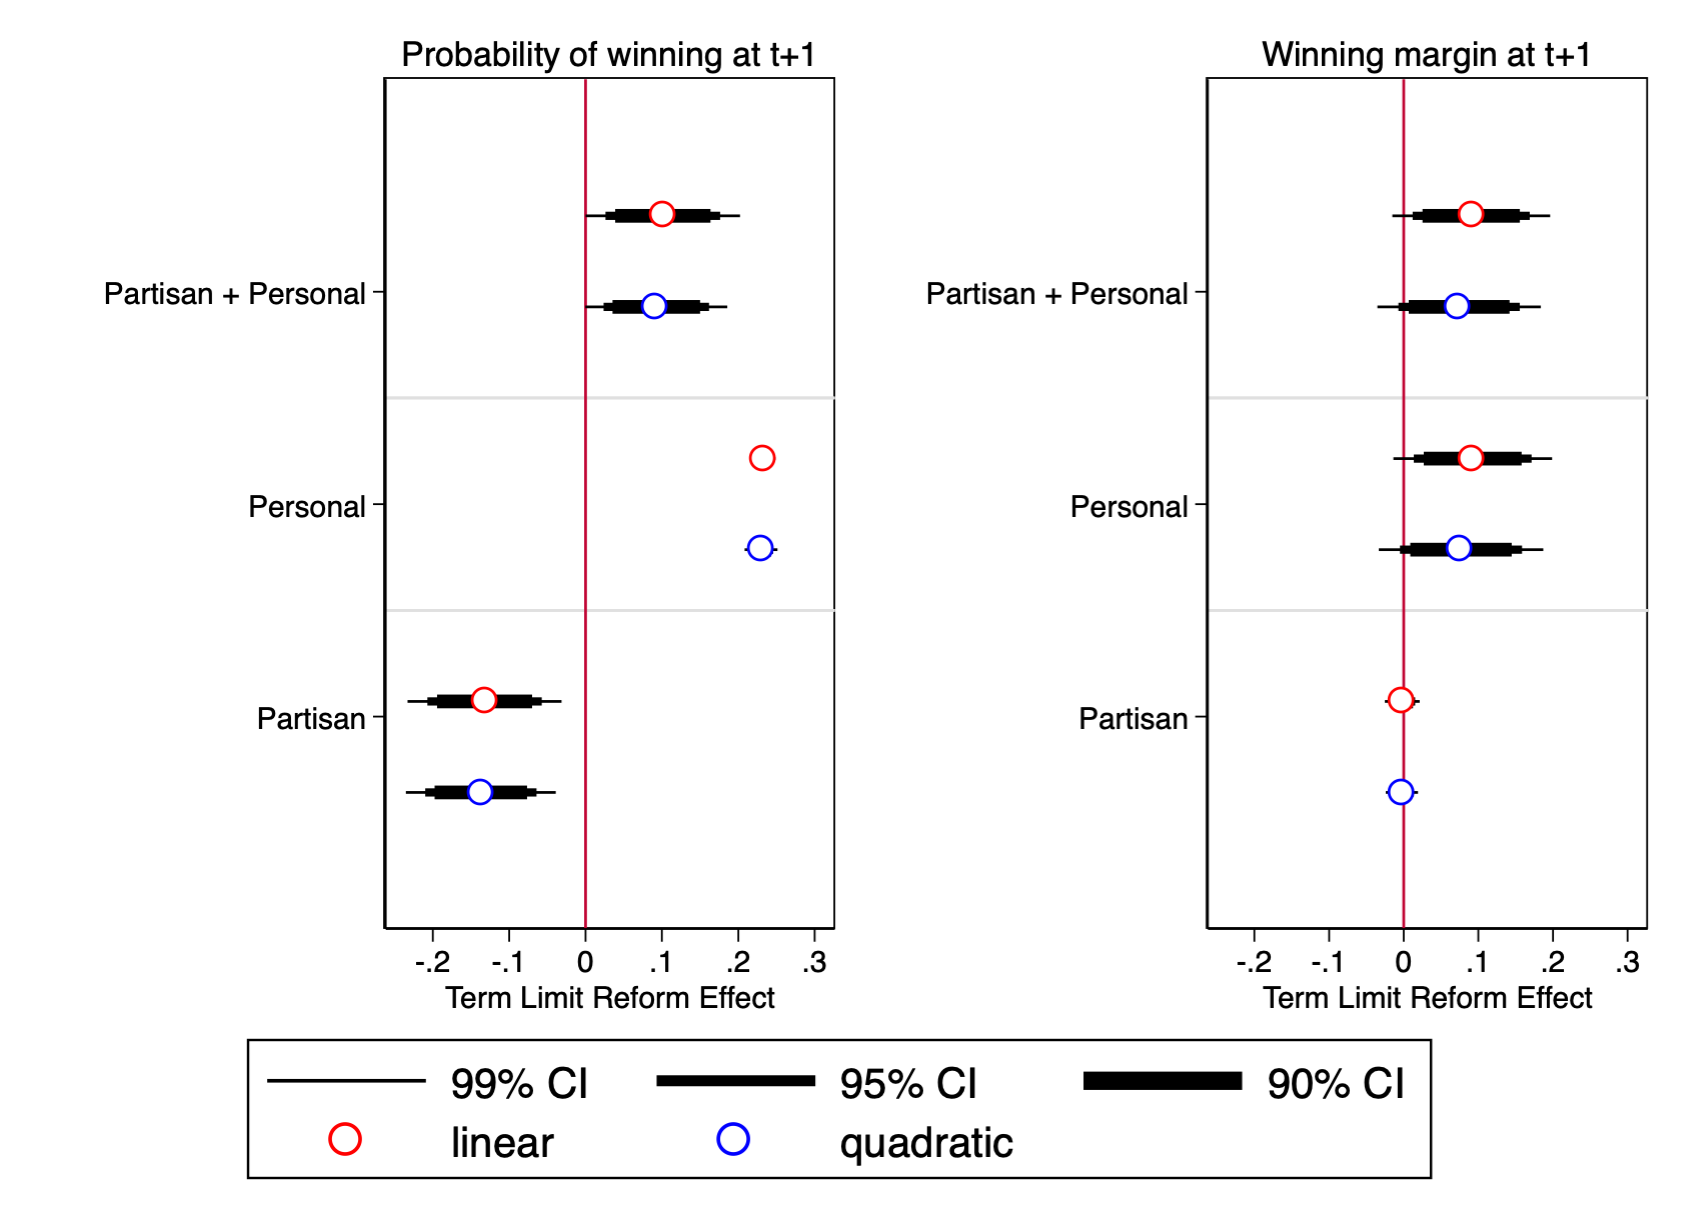
\includegraphics[width=0.9\textwidth]{../Figures_incumbency/twfe_personalvspartisan_advantage.png}
 
  \textbf{Note:} The left panel in figure \ref{fig:twfe_partisan&personal} shows the average treatment effect of the Term Limit Reform on the probability of winning in the following election using a difference in discontinuity of close elections design; the right panel shows the winning margin. Optimal bandwidths following \citet{calonicoetal_2014} are used. This analysis identifies the party that wins at $t-1$ and studies the effect of this party barely winning (or losing) at $t$ on outcomes at election $t+1$ following \citet{klasnja_titiunik_2017}.  
\end{figure} 
\end{comment}

%Figure:
 \begin{figure}[h]   
\centering
 \caption{Personal and Partisan Incumbency Advantage, event study design}
 \label{fig:naive_partisan&personal}
 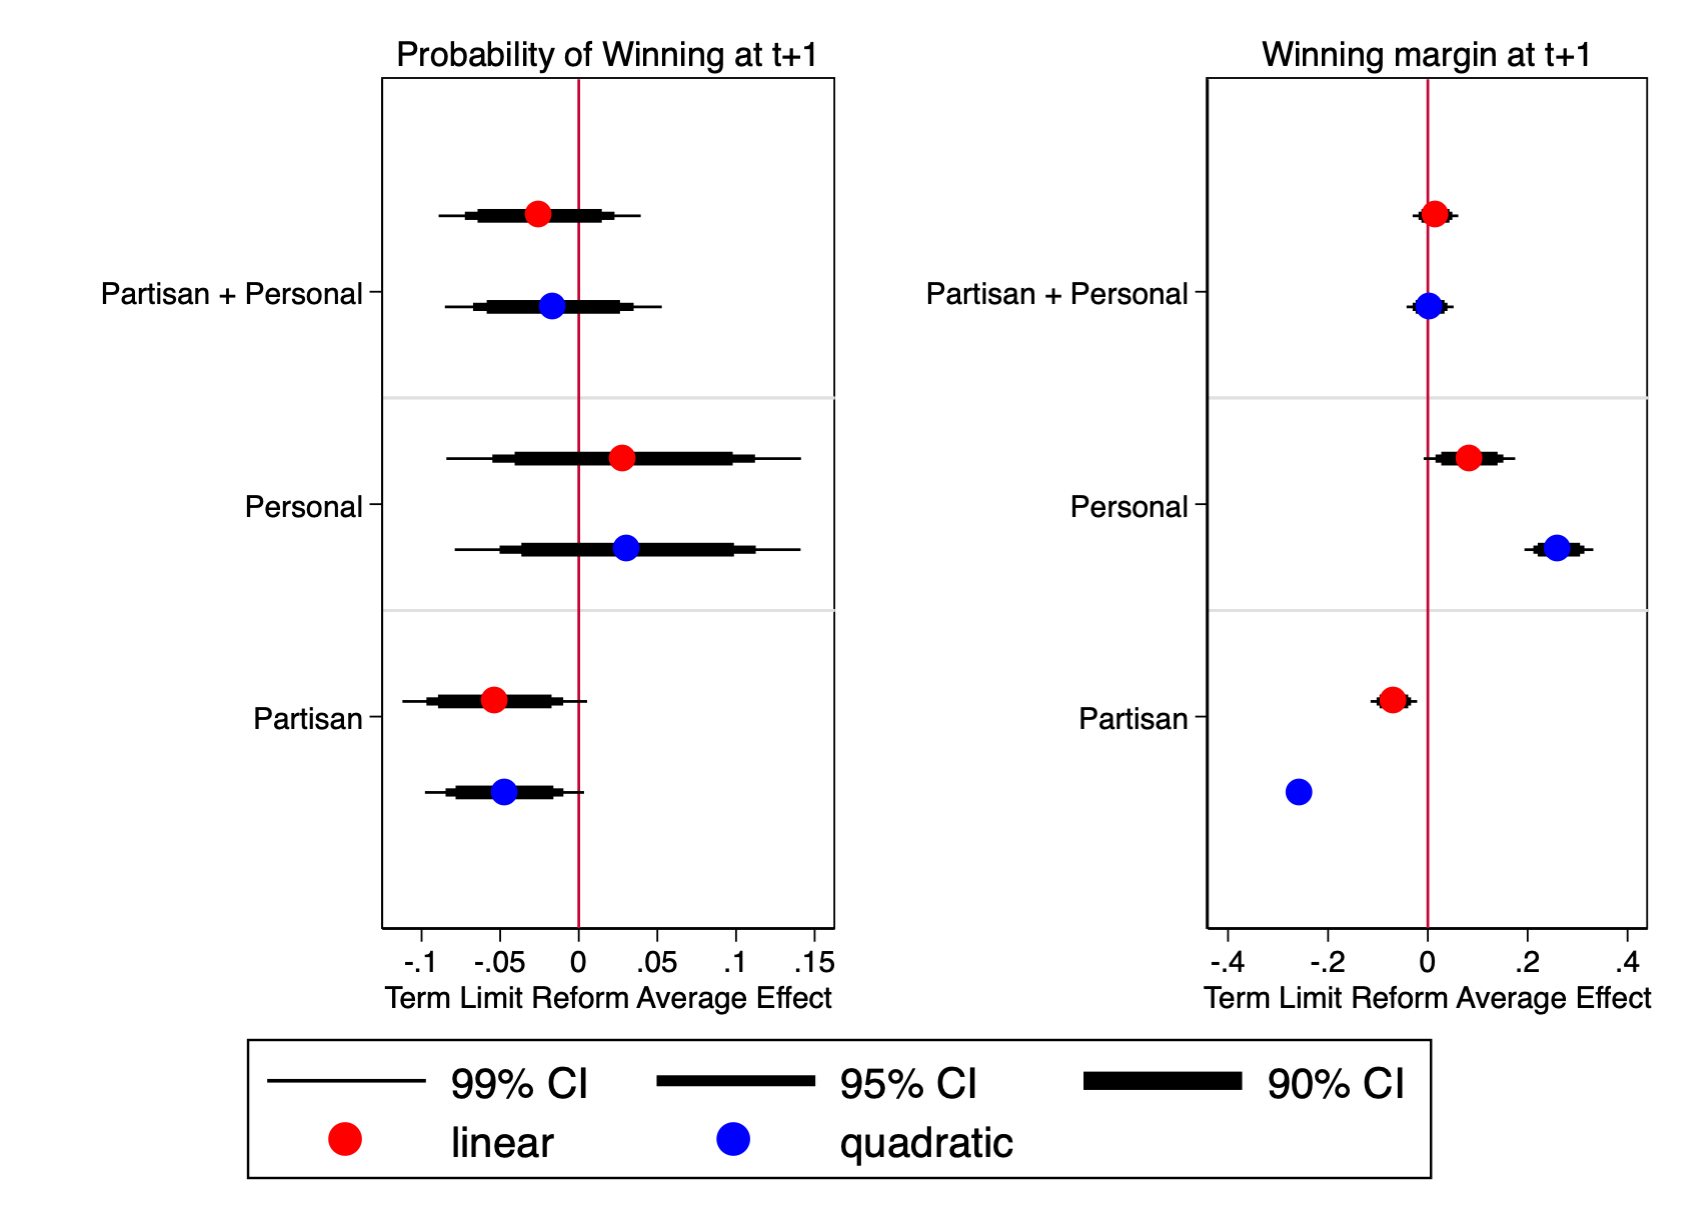
\includegraphics[width=0.9\textwidth]{../Figures_incumbency/naive_personalvspartisan_advantage.png}
 
  \textbf{Note:} The left panel in figure \ref{fig:naive_partisan&personal} shows the average treatment effect of the Term Limit Reform on the probability of winning in the following election using a difference in discontinuity of close elections design; the right panel shows the winning margin. Optimal bandwidths following \citet{calonicoetal_2014} are used. This analysis identifies the party that wins at $t-1$ and studies the effect of this party barely winning (or losing) at $t$ on outcomes at election $t+1$ following \citet{klasnja_titiunik_2017}.  
\end{figure} 
       
\begin{figure}[h]   
\centering    
 \caption{Effect of Term Limit Reform on Partisan and Personal Incumbency Advantage, using winning margin in $t+1$ \\ -difference-in-discontinuity of close elections design-}
 \label{fig:personal_vs_partisan}
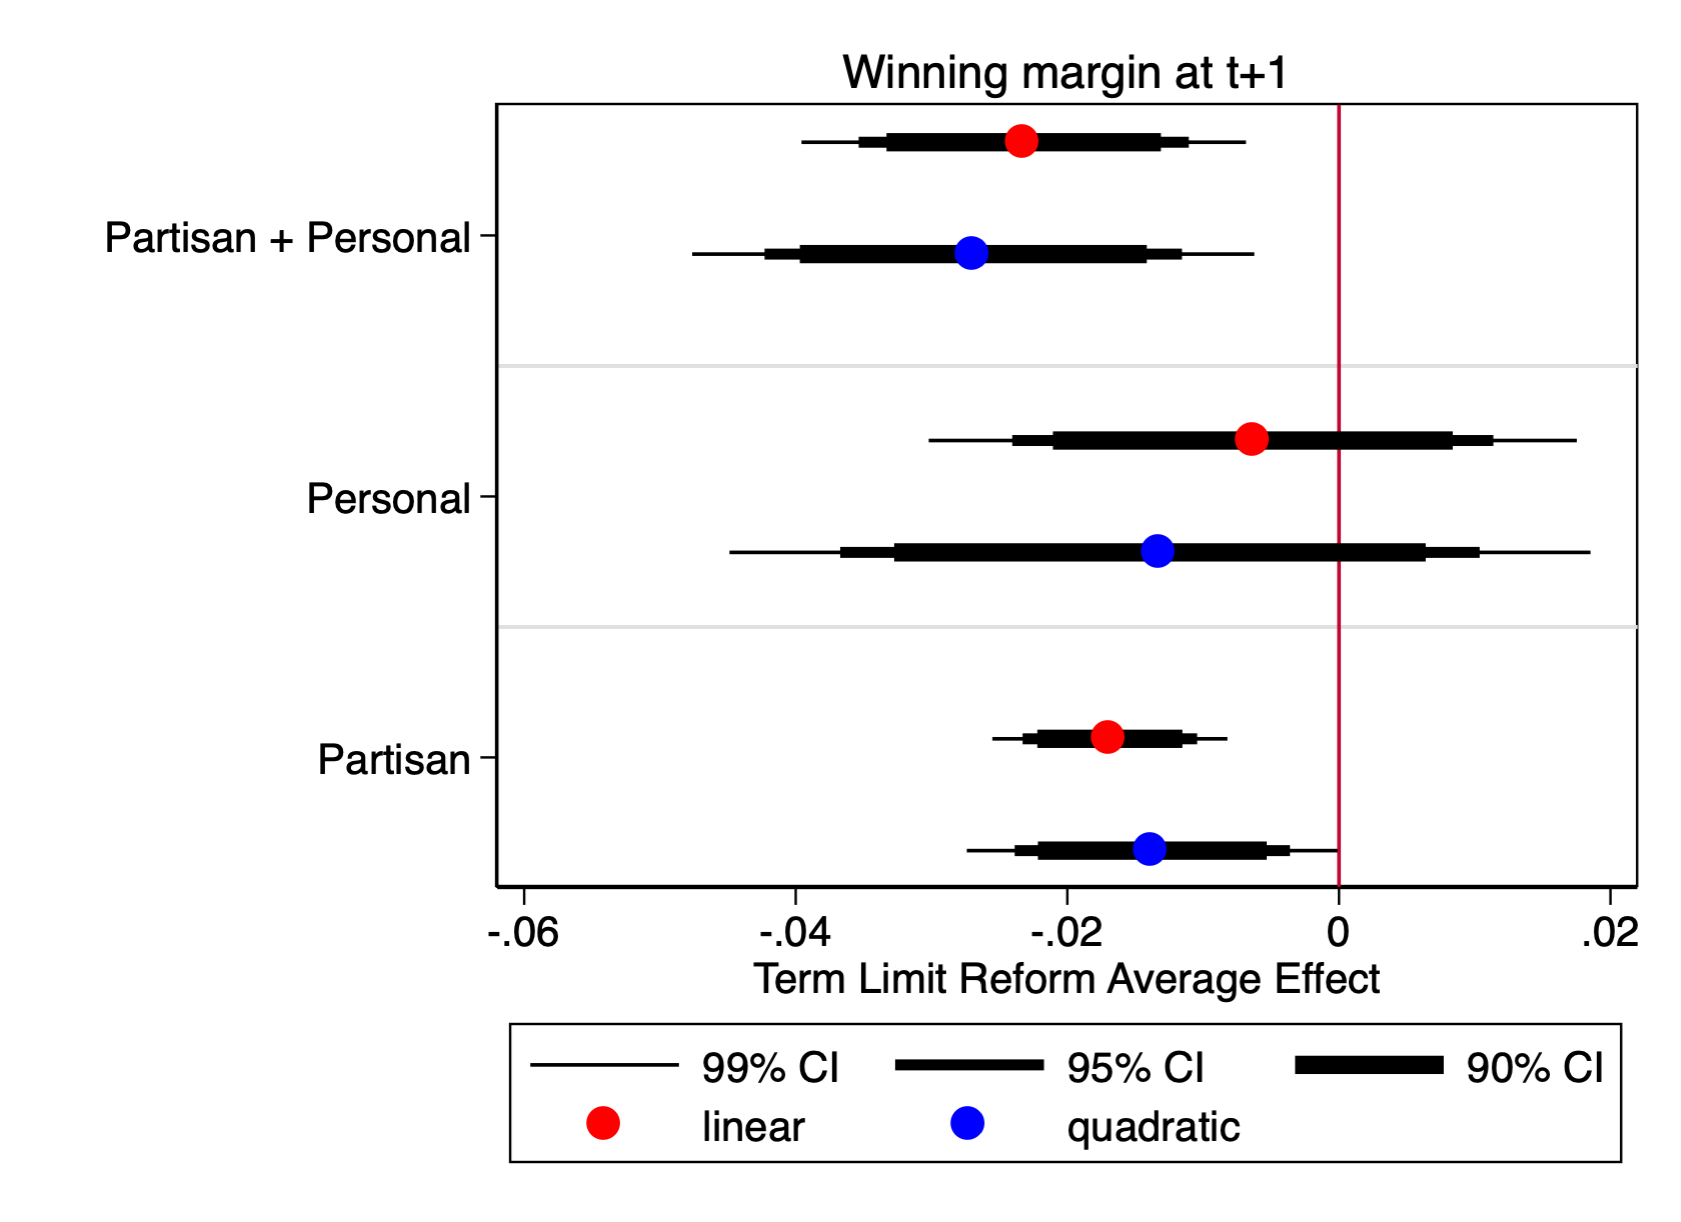
\includegraphics[width=0.9\textwidth]{../Figures_incumbency/partisan_personal_inc_advantage_margin.png}
       \captionsetup{justification=centering}
       
 \textbf{Note:} Figure \ref{fig:personal_vs_partisan} shows the average treatment effect of the Term Limit Reform on the probability of winning in the following election using a difference in discontinuity of close elections design. This average effect was estimated using the IW estimators following \citet{abraham_sun_2020} for each lead and lag relative to the first year a municipality implemented reelection. Optimal bandwidths following \citet{calonicoetal_2014} are used. This analysis identifies the party that wins at $t-1$ and studies the effect of this party barely winning (or losing) at $t$ on outcomes at election $t+1$ following \citet{klasnja_titiunik_2017}. I follow \citet{fowler_hall_2014} to decompose the incumbency advantage into the partisan and personal component. Red and blue points show that parallel trends hold, while hollow ones imply pretrends. 
\end{figure}  
    
    
\begin{figure}[h]   
\centering
 \caption{McCrary Test}
 \label{fig:mcrary}
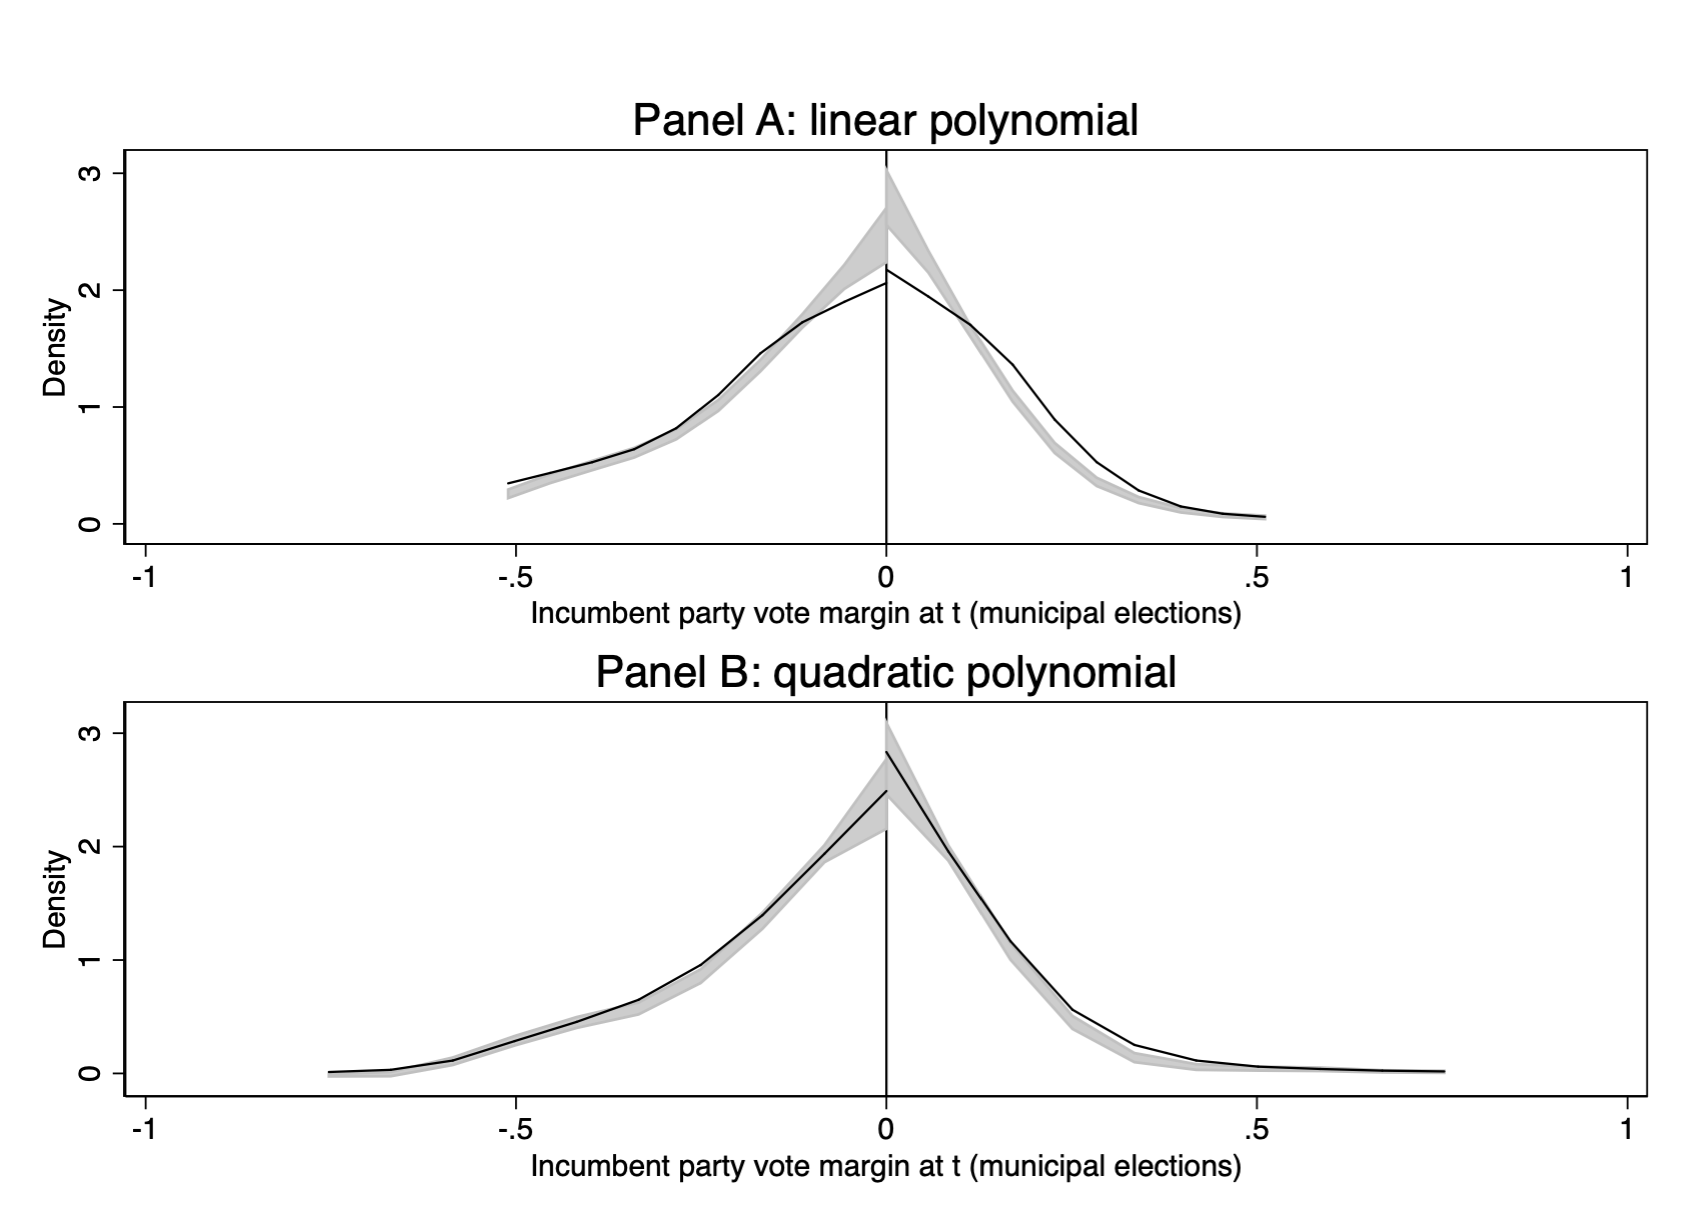
\includegraphics[width=1\textwidth]{../Figures_incumbency/mccrary_pol1_2.png}
%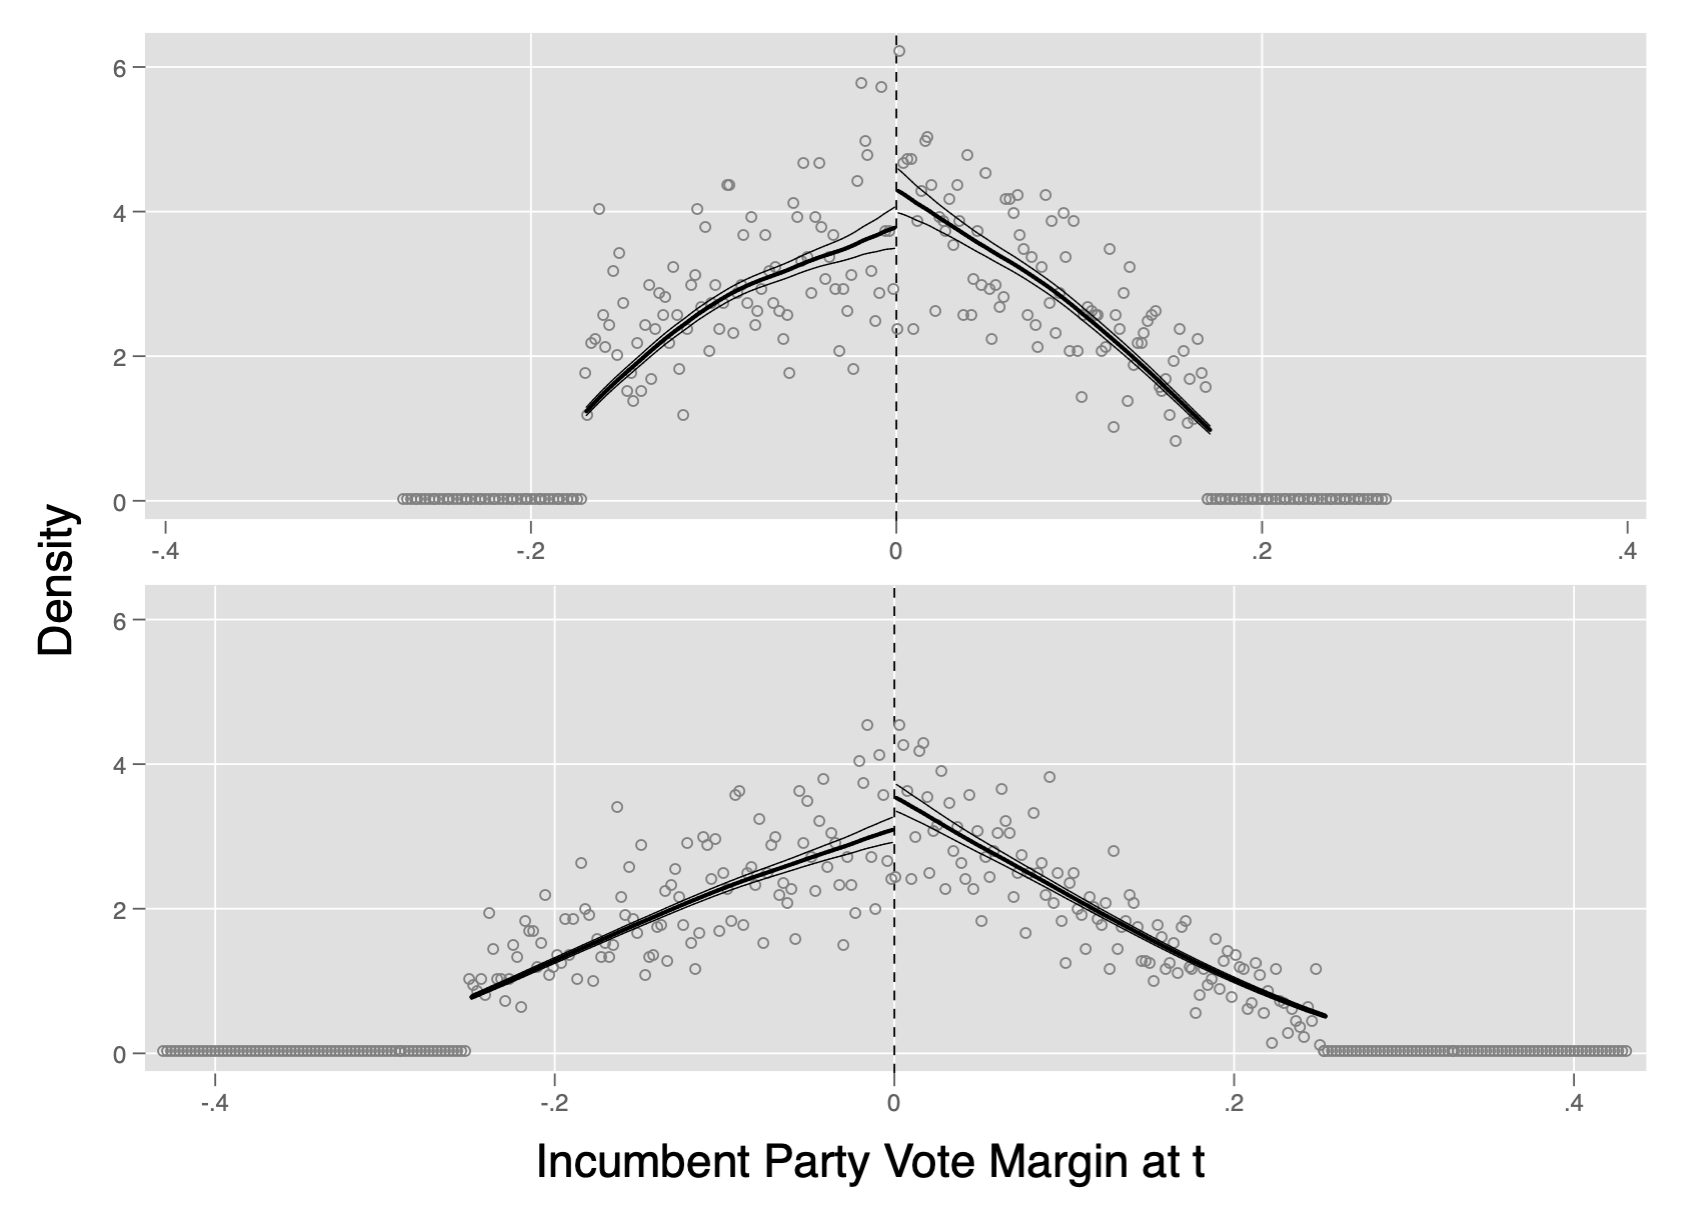
\includegraphics[width=0.9\textwidth]{../Figures/conditional_mccrary_test_pol1_final.png}

       \captionsetup{justification=centering}
         
 \textbf{Note:} 95\% confidence intervals reported.
 
\end{figure} 

 \begin{figure}[h]   
\centering
 \caption{No discontinuous jump of covariates}
 \label{fig:parallel_trend}
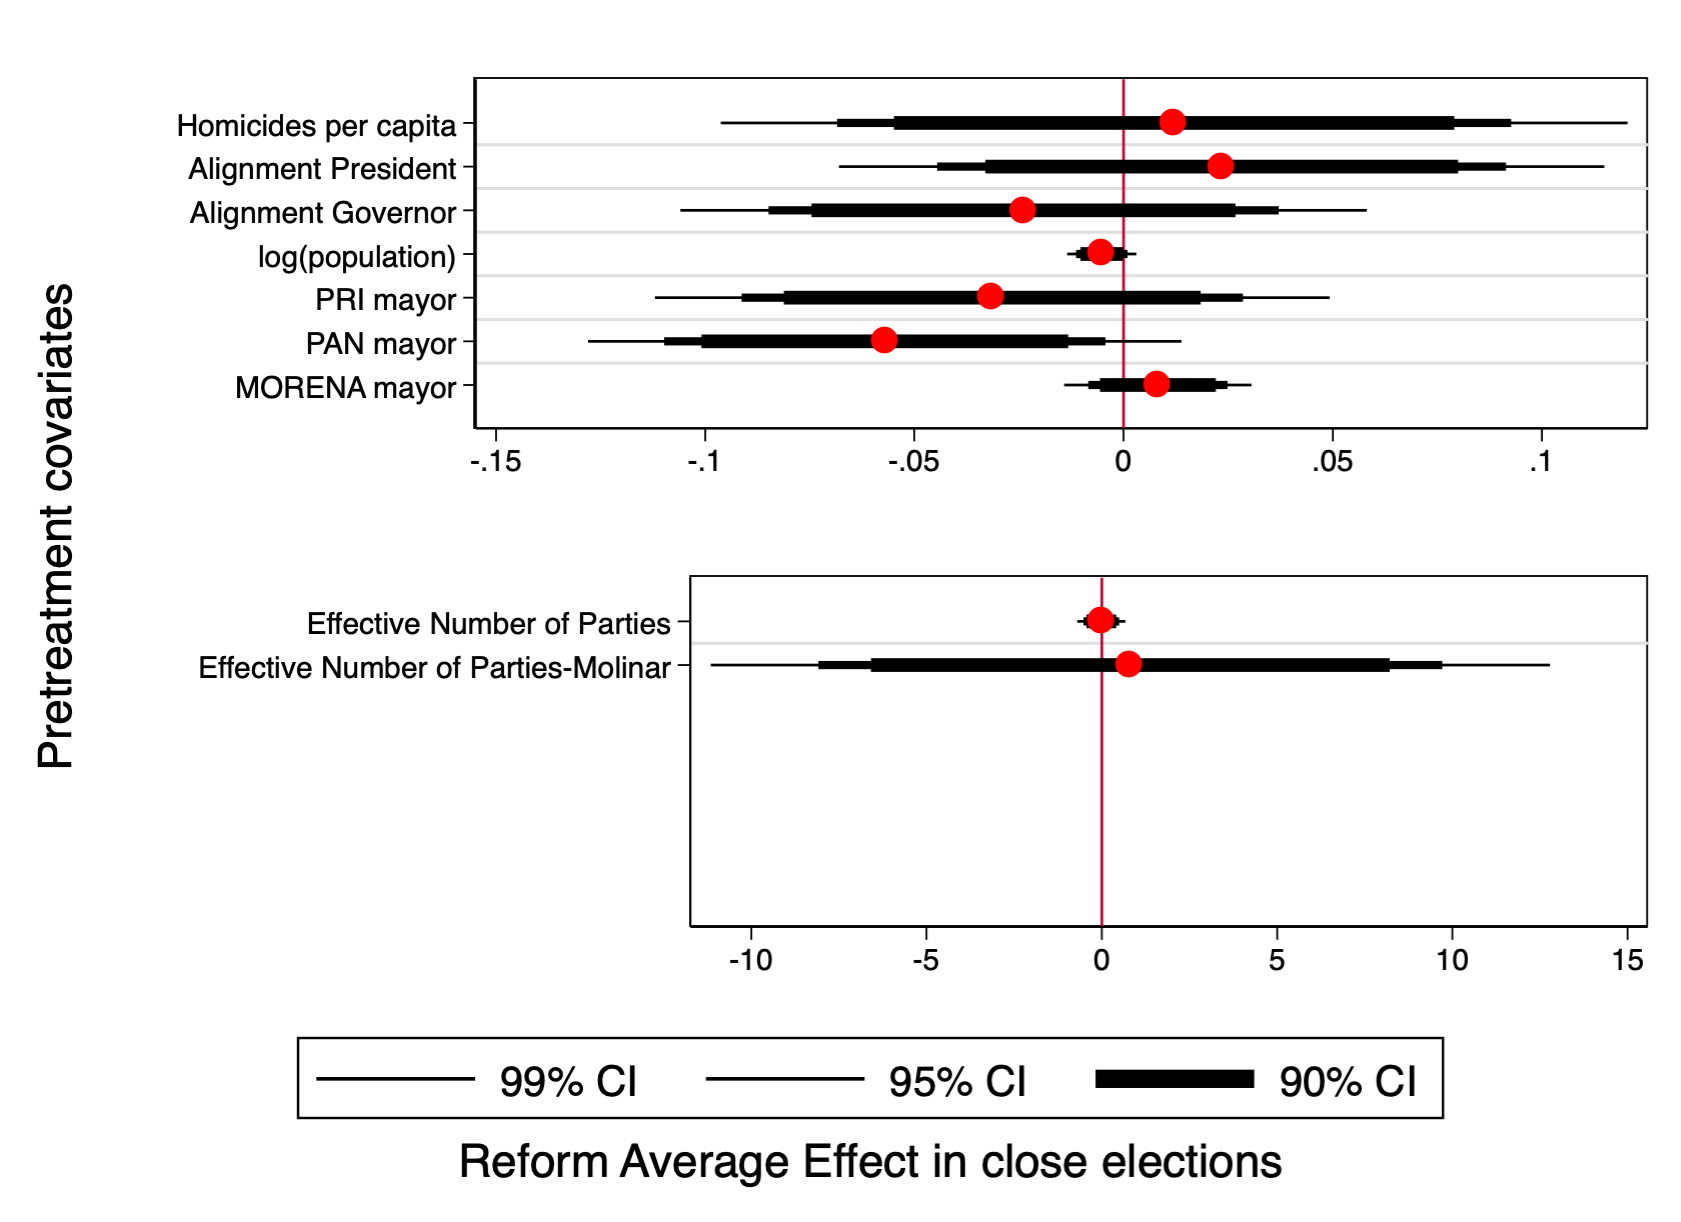
\includegraphics[width=0.9\textwidth]{../Figures/nojump.png}
       \captionsetup{justification=centering}
    
 %\textbf{Note:}.  
   
\end{figure} 


 \begin{figure}[h]   
\centering
 \caption{Testing Different Bandwidths}
 \label{fig:parallel_trend}
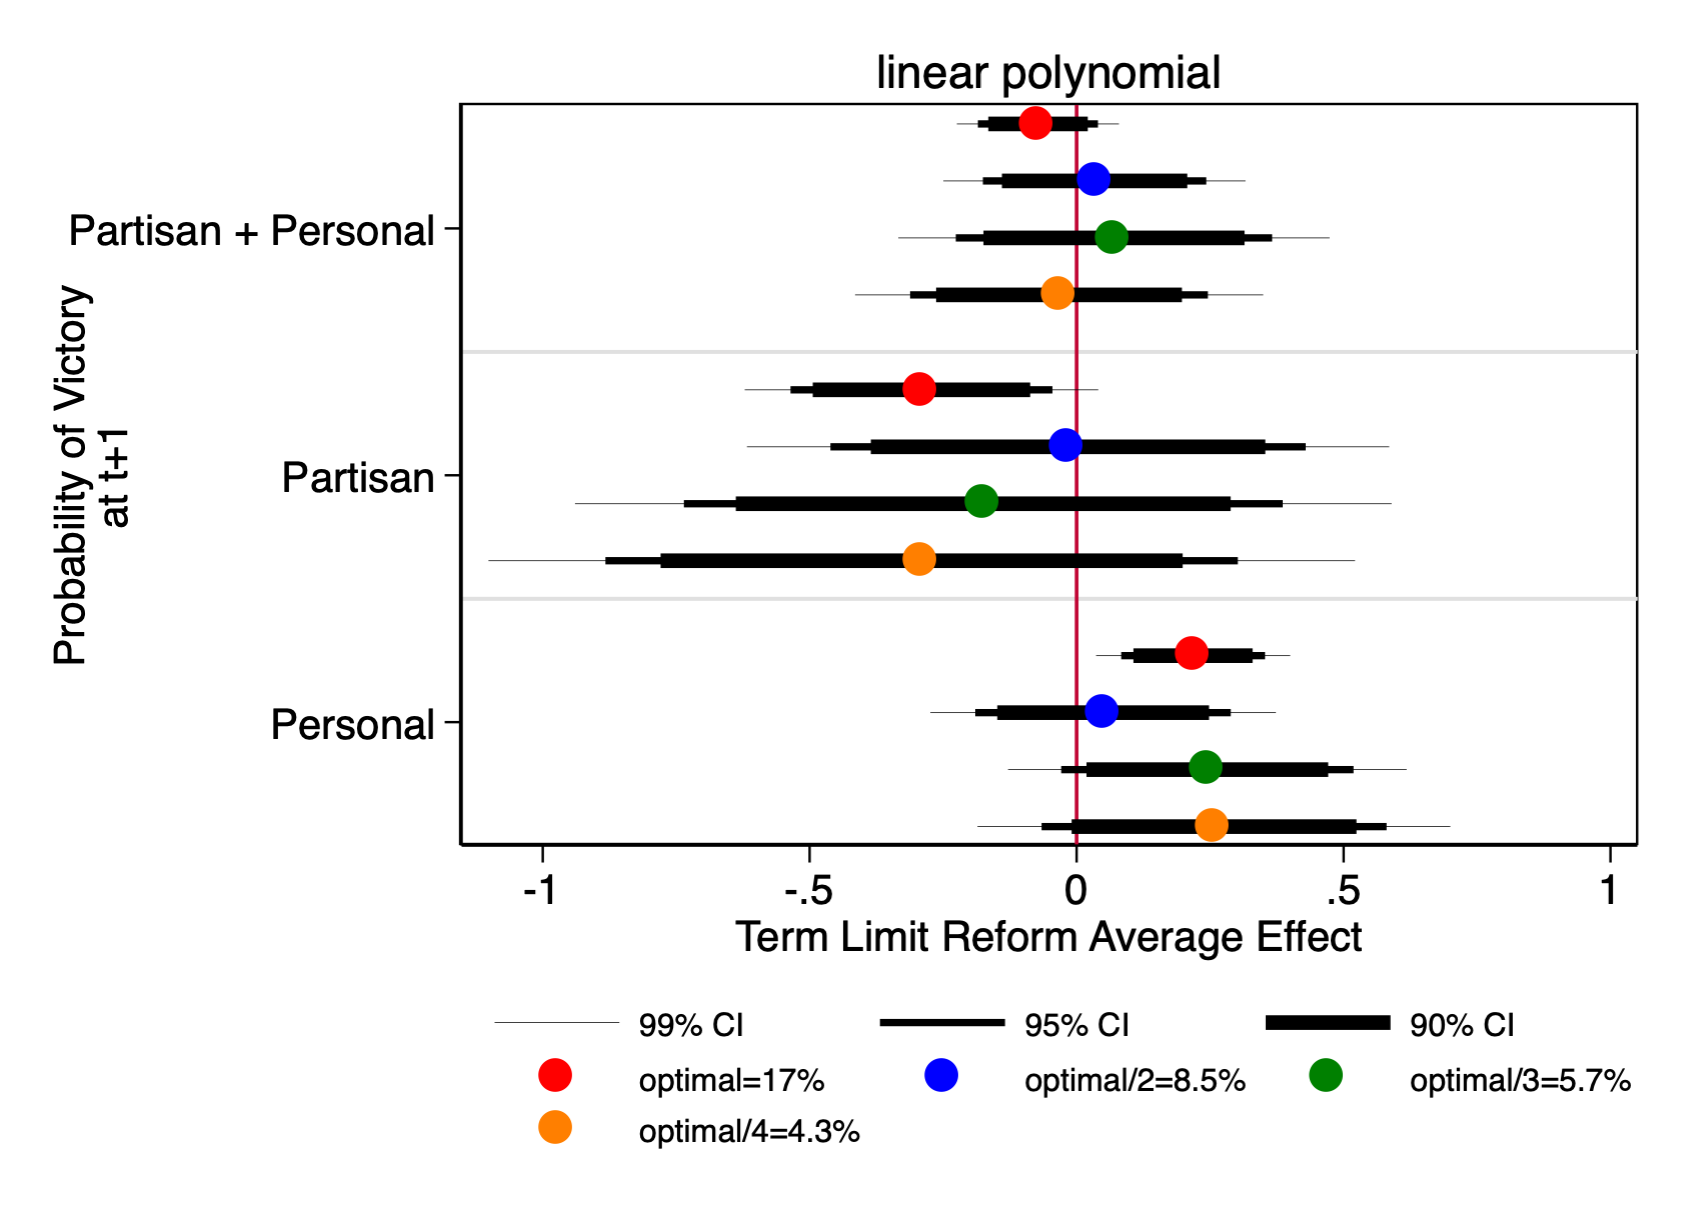
\includegraphics[width=0.9\textwidth]{../Figures/many_bandwidths_linear.png}
       \captionsetup{justification=centering}
 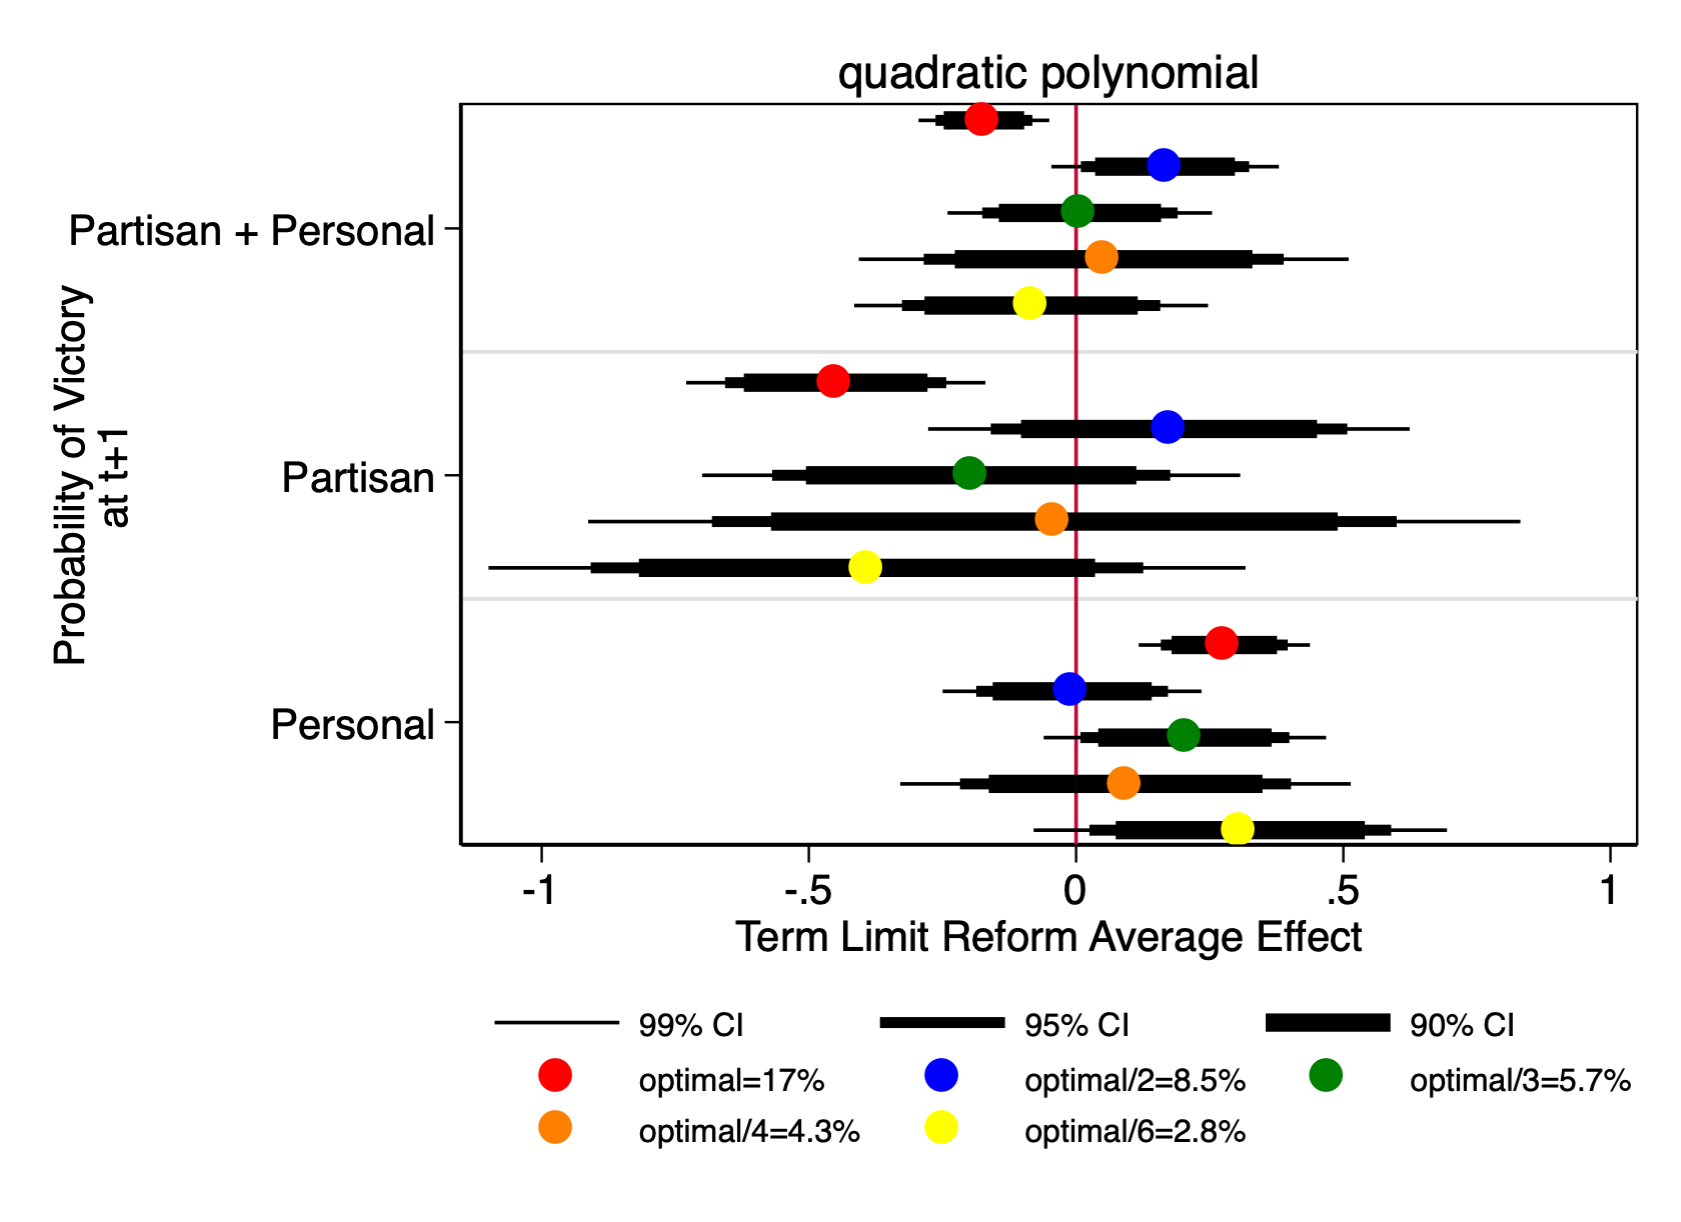
\includegraphics[width=0.9\textwidth]{../Figures/many_bandwidths_quadratic.png}

 %\textbf{Note:}.  
   
\end{figure} 



\begin{figure}[h]   
\centering
 \caption{Effect of Term Limit Reform on Fiscal Transfers, considering only municipalities with close elections}
 \label{fig:resources2}
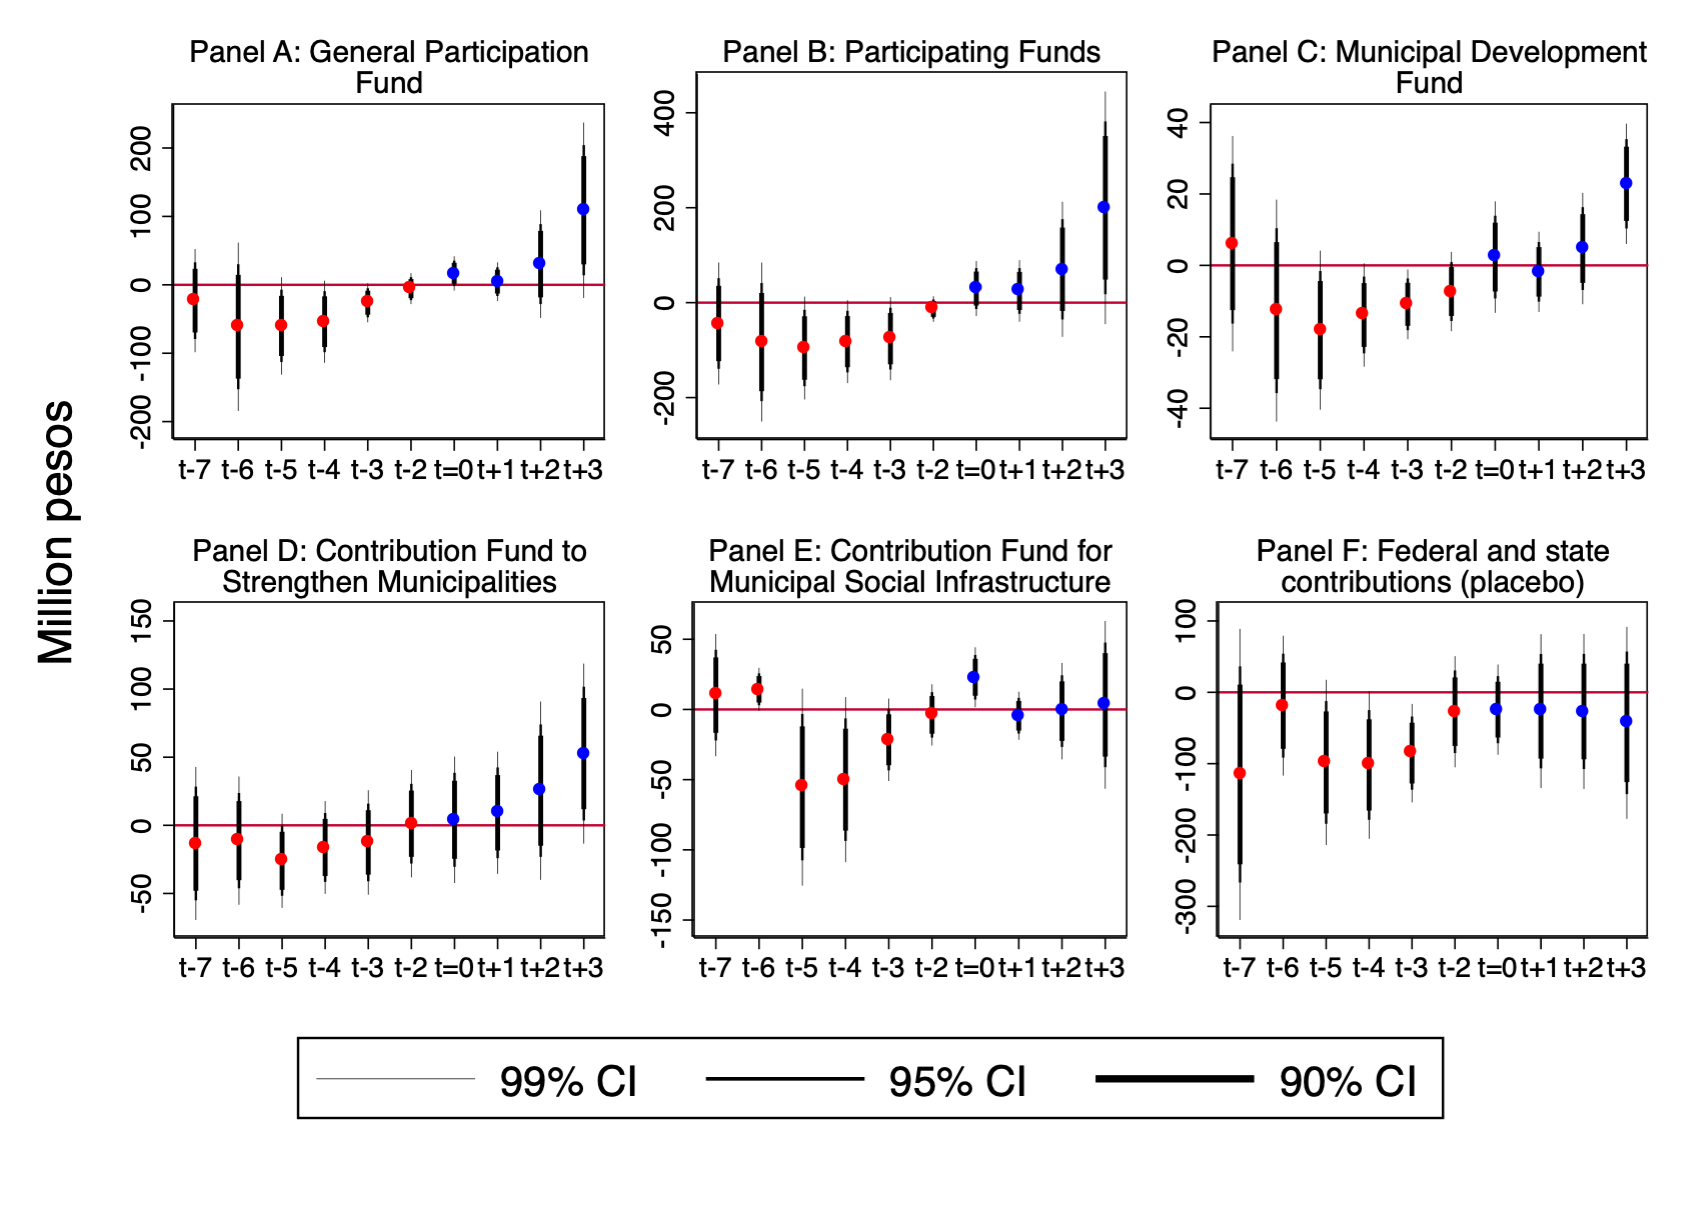
\includegraphics[width=0.9\textwidth]{../Figures_incumbency/resouce_based_incumbency_allyears.png}
       \captionsetup{justification=centering}
         
 \textbf{Note:} Figure \ref{fig:resources2} shows the average treatment effect of the Term Limit Reform on a dummy indicator of whether candidates hold a professional title. This average effect was estimated using the IW estimators following \citet{abraham_sun_2020} for each lead and lag relative to the first year a municipality implemented reelection. Same optimal bandwidths as those in Figure \ref{fig:parallel_trend} are used, as well as the same number of observations.  
       
\end{figure}  

\clearpage
%%%%%%%%%%%%%%%%%%%%%%%%%%%%%%%%% 
%%%% RDD design

 \renewcommand{\thetable}{B-\arabic{table}}
\setcounter{table}{0}
 
\renewcommand{\thefigure}{B-\arabic{figure}}
\setcounter{figure}{0}

\section{Regression Discontinuity Design of close elections, comparing elections with and without term limits \label{appendix:rdd}} 

I begin by visualizing the effect of the reform on incumbency advantage.  Figure \ref{fig:incumbency_advantage} presents the RDD estimate of close elections on incumbency advantage  within an optimal bandwidth distance $h$ from the cutoff (0), and a quadratic polynomial:\footnote{A triangular kernel is used. Results are almost unchanged when using other polynomial functional forms.} Panel A shows a comparison of municipalities with incumbents at $t-1$ that barely won to those that barely lost in $t$ on the probability of electoral victory at $t+1$,\footnote{Incumbency advantage measure following \citet{klasnja_titiunik_2017}.} taking into account all elections from 1979 to 2014 (i.e. prior to the term-limit reform); Panel B shows the same comparison but restricting the sample to municipalities that implemented reelection after 2014. I do not consider those municipal elections that after 2014 did not implement reelection. Table \ref{tab:rdd} shows RD estimates using multiple polynomial functional forms. Even though RD estimates are biased in this setting, especially for Panel B in Figure \ref{fig:incumbency_advantage} (and even columns in Table \ref{tab:rdd}) since in the presence of staggered treatment timing and heterogeneous treatment effects across cohorts are not causally interpretable since we are considering both early vs late adopters of the reform on the treated,\footnote{The next iteration of this working paper will show this proof in the Appendix for RD designs.} they provide a striking depiction of what occurred before and after the electoral reform. 


\begin{figure}[H]
\centering
\caption{Effect of Term Limit Reform on Incumbency Advantage, quadratic polynomial}
  \label{fig:incumbency_advantage} 

	{\textbf Figure A: Probability of winning at t+1}
	 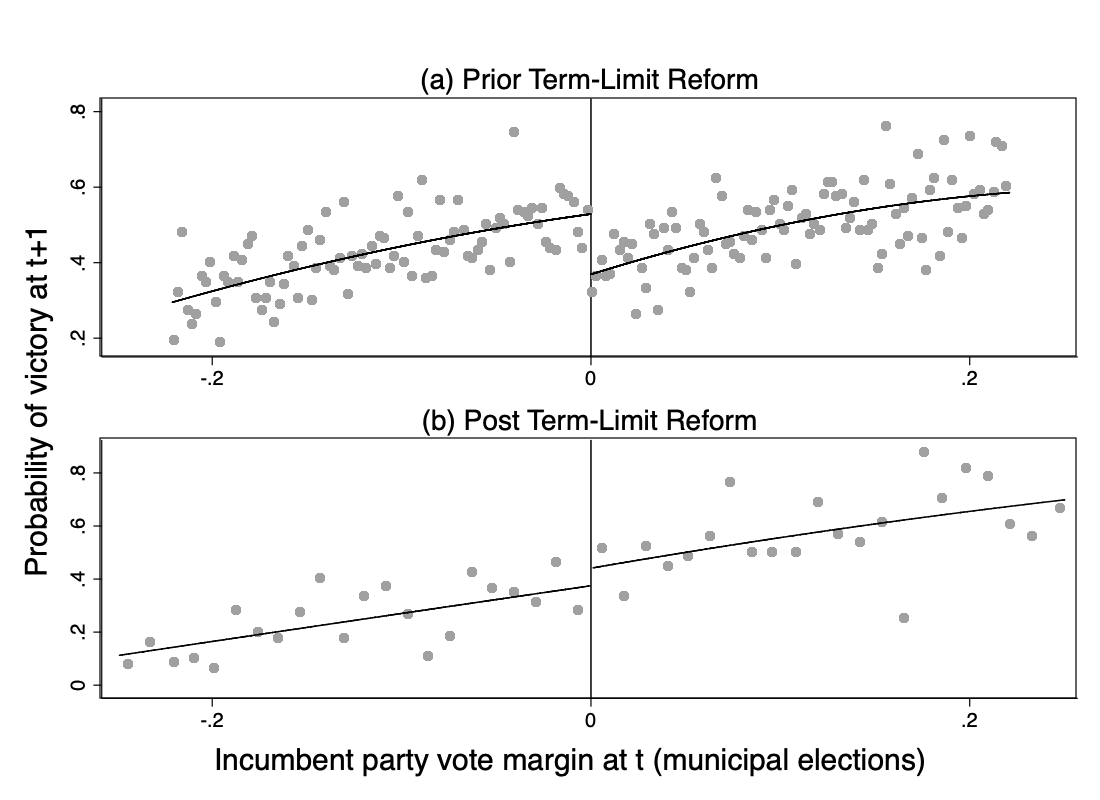
\includegraphics[width=0.6\textwidth]{../Figures_incumbency/RDD_incumbency_pol2.png}
	 \\
	{\textbf Figure B: Winning margin at t+1}

 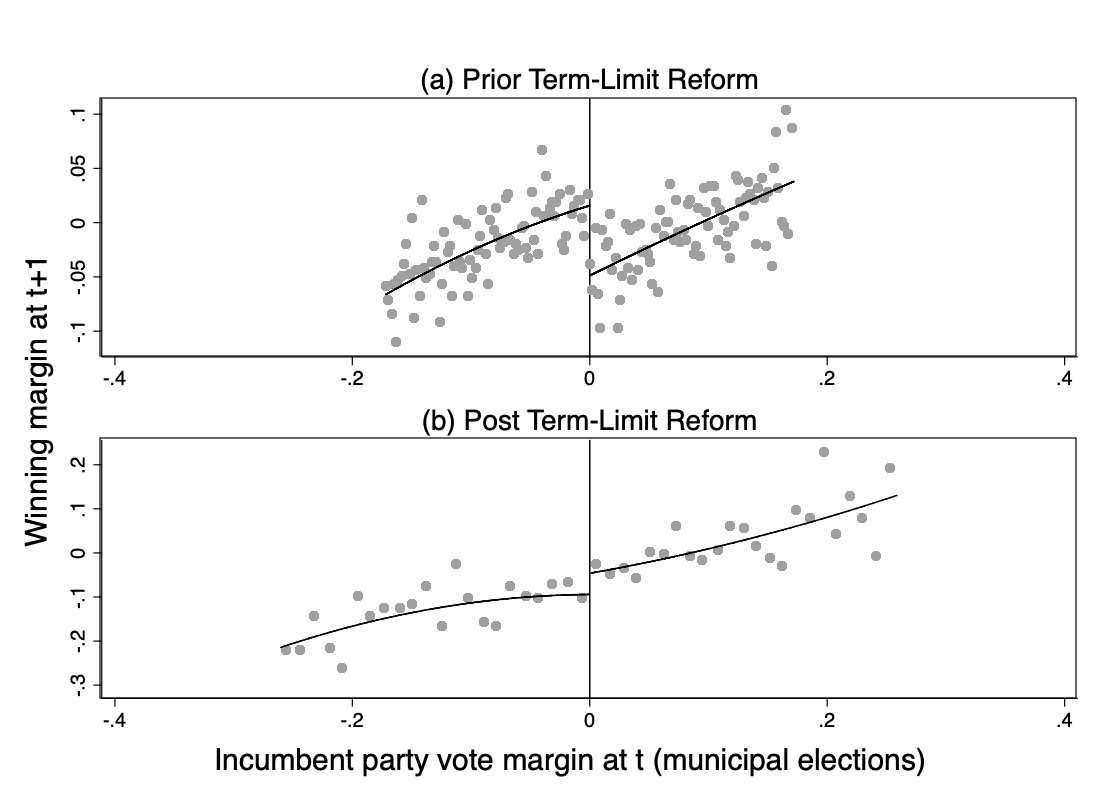
\includegraphics[width=0.6\textwidth]{../Figures_incumbency/RDD_incumbency_margin_pol2.png}
     \captionsetup{justification=centering}  
       
\end{figure} 
       Note: Regression Discontinuity design of close elections on incumbency advantage. Panel (a) considers all elections from 1979 to 2014. Panel (b) considers all elections after 2014 for municipalities that implemented reelection.) 
\\
       
Before the reform, there was a negative statistical significant difference between municipalities that barely won and lost on the probability of success in the next election. This incumbency \emph{disadvantage} aligns strongly with a similar result found by \citet{klasnja_titiunik_2017} for the case of Mexico. \citet{klasnja_titiunik_2017} find that an incumbent party that is barely reelected suffers a reduction in the probability of winning the following election of 28 percentage points. In contrast, I find a reduction between 10.7 to 11.32 percentage points, a finding that considers 20 more years of elections since \citet{klasnja_titiunik_2017} cap their data from 1997 to 2009, while I consider elections since 1979 to 2014. 

More interesting is the finding that after reelection takes place the previous incumbency disadvantage disappears as noted by a positive and non-statistical significant difference between municipalities that barely lost and won an election. This initial RDD results provide suggestive evidence that the electoral reform generated an increase in the probability of victory in the next election for municipalities that barely won an election relative to those that barely lost. These estimates, however, may be biased. By comparing term limit and non-term limit elections we are assuming there are parallel trends for identification which might not be the case. Furthermore, as \citet{eggers_2017} even when comparing close elections, a potential difference in the quality of incumbents and challengers may exist. 
 
 \\ 
  
%Table:
\begin{table}[!htbp]\def\sym#1{\ifmmode^{#1}\else\(^{#1}\)\fi}
\caption{Regression Discontinuity Design of Close Elections on Incumbency Advantage: Comparison of term and non-term limited elections}
\label{tab:rdd}
\begin{center} 
\scalebox{1}{
\begin{tabular}{lcccc}
 
\hline \hline   
\\       
   
\multicolumn{5}{l}{Dependent variable:}\\
  
\\
            &\multicolumn{2}{c}{linear polynomial}      &\multicolumn{2}{c}{quadratic polynomial}   \\\cmidrule(lr){2-3}\cmidrule(lr){4-5}
            &\multicolumn{1}{c}{(1)}         &\multicolumn{1}{c}{(2)}         &\multicolumn{1}{c}{(3)}         &\multicolumn{1}{c}{(4)}         \\
\addlinespace
Probability of victory at t+1&      0.0711         &     -0.1589\sym{***}&      0.0554         &     -0.1616\sym{***}\\
            &    (0.0636)         &    (0.0260)         &    (0.0846)         &    (0.0323)         \\
\addlinespace
Observations&         887         &       6,072         &         954         &       7,287         \\
Term Limit  &                     &  \checkmark         &                     &  \checkmark         \\
 
\\
            &\multicolumn{2}{c}{linear polynomial}      &\multicolumn{2}{c}{quadratic polynomial}   \\\cmidrule(lr){2-3}\cmidrule(lr){4-5}
            &\multicolumn{1}{c}{(1)}         &\multicolumn{1}{c}{(2)}         &\multicolumn{1}{c}{(3)}         &\multicolumn{1}{c}{(4)}         \\
\addlinespace
Winning margin at t+1&      0.0307         &     -0.0452\sym{***}&      0.0390         &     -0.0463\sym{***}\\
            &    (0.0305)         &    (0.0081)         &    (0.0343)         &    (0.0102)         \\
\addlinespace
Observations&         677         &       7,328         &         955         &       9,157         \\
Term Limit  &                     &  \checkmark         &                     &  \checkmark         \\
 
 
                 
\hline \hline   
\multicolumn{5}{p{0.8\textwidth}}{\footnotesize{Notes: Standard errors in parentheses, with the following significance-level: $^{***}$ 1\%; $^{**}$ 5\%; and $^*$ 10\%, that refer to two-sided t-test. Optimal bandwidth following \citet{calonicoetal_2014} $^a$ Incumbency advantage measured following \citet{klasnja_titiunik_2017}. 
  }} \\  
\end{tabular}         
}
\end{center} 
\end{table} 

\clearpage
  
\end{document}
